\documentclass[11pt]{article}
\usepackage[margin=1in]{geometry}
\usepackage{booktabs}
\usepackage{graphicx}
\usepackage{amsmath}
\usepackage{amssymb}
\usepackage{xcolor}
\usepackage{microtype}
\usepackage{placeins}
\usepackage[authoryear,round]{natbib}
\usepackage[colorlinks=true,citecolor=blue!60!black,linkcolor=blue!60!black,urlcolor=blue!60!black]{hyperref}

\title{Hand-to-Mouth Households in Uzbekistan:\\Survey Forensics, Income Risk, and a Three-State Markov-TANK Calibration, 2018--2025}
\author{Utkirbek Azimov\thanks{PhD Candidate, Termez State University, Termez, Uzbekistan. Email: \texttt{azimov2398@gmail.com}. ORCID: \href{https://orcid.org/0000-0002-8088-324X}{\texttt{0000-0002-8088-324X}}. Working Paper / Preprint v1.0.0. Replication package: \url{https://github.com/azimovu/uzbekistan-hank-lite}.}}
\date{November 2026}

\begin{document}
\maketitle
\vspace{-1.0em}

\begin{abstract}
We measure hand-to-mouth (HtM) behavior, income risk, and shock exposure in Uzbekistan using 82 consecutive monthly rounds of the World Bank's Listening to Citizens of Uzbekistan (L2CU) phone panel, covering 2,499 households and 121,618 household-rounds from September 2018 to June 2025. An audit of the survey instrument uncovers four discontinuities that distort raw HtM series: two recording breaks in savings drawdowns, a round-29 drop in reported food-consumption cuts, and a post-round-43 food-sufficiency anomaly among untouched savers. Harmonizing these items puts pooled broad HtM at 59.9\% (61.3\% when imputing break windows) and strict HtM at 15.5\%, peaking in April 2020 at 73.7\% and 30.8\%. Filtering phone-survey classification noise with a population-weighted three-state hidden-Markov model reveals persistent underlying states (17- to 41-month expected spells) and a latent broad-HtM share of 65.7\% (60.6\% starting post-trough at round 36; 70.3\% under break-window imputation; 62.4\% excluding food cuts). Matching CPI-deflated log-income autocovariances yields persistent monthly risk ($\rho_z = 0.923$), invariant across agricultural and non-agricultural households. Linked labor records show that strict-HtM households lose work four to five times as often as savers even at two- to three-month lags. Embedded in a partial-equilibrium, intertemporal-budget-constraint-consistent microsimulation, these moments imply steady-state pass-through of 0.59--0.63 at $m_M = 1.00$ (0.52--0.56 at $m_M = 0.85$; 0.36--0.40 at $m_M = 0.50$) and show that regressive job-loss incidence amplifies an equal-aggregate-loss $-10\%$ income contraction by 1.26$\times$ to 1.40$\times$ on impact (rising to 1.73$\times$ at $m_M = 0.50$).
\end{abstract}

\medskip\noindent
\textbf{JEL codes:} E21, E32, D31, O12, P36.

\medskip\noindent
\textbf{Keywords:} hand-to-mouth households, TANK, marginal propensity to consume, income risk, matching multiplier, Uzbekistan.

\section{Introduction}\label{sec:intro}

Aggregate spending falls most sharply during a downturn when households lack liquid buffers, and deeper still when income losses fall heavily on families with high marginal propensities to consume \citep{campbell1989consumption,gali2007understanding,bilbiie2008limited,kaplan2018monetary,achdou2022income}. In two-agent and heterogeneous-agent New Keynesian (TANK and HANK) models, the hand-to-mouth (HtM) share and the timing of spending responses govern both fiscal multipliers and monetary transmission \citep{werning2015incomplete,auclert2019monetary,bilbiie2020new,auclert2024intertemporal,debortoli2025heterogeneity}. Earlier studies linked high marginal propensities to consume (MPCs) to borrowing limits and buffer-stock saving \citep{zeldes1989consumption,jappelli1990consumption,carroll1997buffer}, while \citet{kaplan2014model}, \citet{kaplan2014wealthy}, and \citet{aguiar2025hand} showed that illiquid balance sheets can leave even higher-income households hand-to-mouth. Empirical work on tax rebates, lotteries, cash transfers, and administrative registries confirms wide MPC dispersion \citep{sahm2010household,parker2013consumer,jappelli2014fiscal,fagereng2021mpc,fuster2021what,egger2022general,kaplan2022mpc,crawley2023consumption}. Related studies of earnings dynamics document partial insurance against persistent shocks \citep{blundell2008consumption,aguiar2015has,arellano2017earnings}, and \citet{patterson2023matching} shows how regressive shock incidence generates a ``matching multiplier'' that deepens recessions.

Most of this evidence comes from advanced economies with bank-account registries or longitudinal expenditure diaries. In developing and post-Soviet transition economies, high-frequency household panels are scarce \citep{deaton1992understanding,townsend1994risk,morduch1995income}. Across Central Asia and the Commonwealth of Independent States (CIS), households rely heavily on cash held at home, cross-border migrant remittances, and newer retail payment cards \citep{kakhkharov2017transaction,seitz2019migration,abduvaliev2020impact,kakhkharov2021south}. Uzbekistan offers a rare empirical window into such an economy. Although no public longitudinal consumption diary exists, the World Bank has fielded the Listening to Citizens of Uzbekistan (L2CU) monthly household phone panel without interruption since September 2018 \citep{WB2025L2CU}. Linking 82 consecutive monthly waves through June 2025 to individual labor records and official monthly consumer price indices \citep{StatUz2026CPI} allows us to track liquidity status, income risk, and job-loss shocks at monthly frequency over seven years.

Using a seven-year phone panel requires auditing the survey instrument before modeling. Our first contribution is a forensic audit of L2CU's savings and coping items, cross-checked against the World Bank Catalog 6412 metadata \citep{WB2025L2CU}. Naive HtM measures built directly from raw columns contain severe breaks. Two abrupt jumps in reported savings drawdowns (rounds 58--65 and 78--79) pull 79.8\% and 57.1\% of new drawdown reports out of households that had reported zero savings one month earlier. In addition, starting in April 2022 (round 44), households reporting untouched savings suddenly report insufficient food money at rates up to 61.3\%, even though their Food Insecurity Experience Scale (FIES) rate is less than half that of untouched savers reporting sufficient food (6.9\% versus 15.9\%). Harmonizing these discontinuities puts Uzbekistan's broad HtM share at 59.9\% (61.3\% with break-window imputation) and strict HtM at 15.5\%, leaving the April 2020 COVID-19 lockdown as the clear peak of liquidity distress (73.7\% broad, 30.8\% strict).

Our second contribution measures liquidity persistence and monthly earnings risk. Raw monthly transitions across Savers ($S$), non-strict HtM ($M$), and strict HtM ($H$) exhibit heavy churn: nearly half of households observed moving from $S$ to $M$ return to $S$ the following month, pointing to phone-survey classification error \citep{abowd1985effects}. Estimating a population-weighted three-state hidden-Markov model (HMM) on the post-round-29 regime separates reporting noise from true state persistence. Underlying liquidity states last much longer than raw transitions suggest, with expected spells of 31.2 months for savers, 40.8 months for non-strict HtM, and 17.4 months for strict HtM, and a latent broad-HtM share of 65.7\% (ranging from 60.6\% starting post-trough at round 36 to 70.3\% under break-window imputation, and 62.4\% when dropping the food-cut item across all 82 rounds). On the income side, matching CPI-deflated real log-income autocovariances out to lag 24 \citep{blundell2008consumption,guvenen2009empirical} attributes 52.6\% of variance to permanent heterogeneity, 21.3\% to persistent monthly shocks ($\rho_z = 0.923$, half-life 8.7 months), and 26.1\% to transitory or measurement noise. Splitting the panel by agricultural income uncovers a 12-month harvest-cycle wave among agricultural households, yet persistent-shock parameters remain virtually identical across agricultural ($\rho_z = 0.921$) and non-agricultural ($\rho_z = 0.924$) households. Aggregate income shares are also invariant to household-level weights, equivalence scales, 99\% winsorization, and the addition of foreign remittances (7.2\% of total income).

Our third contribution tests whether the intermediate $M$ state, 92.6\% of which consists of households reporting no savings and no active coping ($M_1$), differs behaviorally from savers, and measures who absorbs job losses. Across independent cross-sectional markers in L2CU, $M_1$ households experience roughly double the food insecurity of savers, 2.7 times the utility arrears, and less than half the rate of realized past-30-day saving. When a household member loses work, $M_1$ households increase emergency borrowing by significantly more than savers (+13.1 versus +7.7 percentage points, $t = 2.17$), while post-job-loss food insecurity and weekly flour-spending elasticities are directionally higher for $M_1$ without reaching statistical significance against $S$. Linking household and individual files (118,907 household-rounds) shows that strict-HtM households suffer job loss 4.9 times as often as savers at lag $t-1$, and still 4.0 to 4.1 times as often when liquidity status is lagged two or three months to rule out anticipation. Job loss reduces real household income by 21.8\% to 27.9\%, leaves a visible earnings scar six to twelve months later, and raises broad-HtM entry among affected savers by 22.9 percentage points (14.6 percentage points with household fixed effects).

Finally, we embed these empirical moments in a partial-equilibrium, intertemporal-budget-constraint (IBC)-consistent three-state Markov-TANK microsimulation. Because L2CU lacks a total-consumption diary and liquid-asset balances, state-level MPCs cannot be estimated directly. We therefore calibrate them over an explicit grid ($m_S \in [0.03, 0.15]$, $m_M \in [0.50, 1.00]$, $m_H = 1.00$) and compare smoothed buffer rebuilding against no-borrowing clawback, HMM latent persistence, forward-looking intertemporal MPC (iMPC), and fixed-status permanent-income benchmarks. At $m_S = 0.07$ and $m_M = 1.00$, steady-state aggregate MPCs are 0.628 for lump-sum transfers and 0.586 for proportional shocks (0.560 and 0.520 at $m_M = 0.85$; 0.404 and 0.364 at $m_M = 0.50$). Distributing a $-10.0\%$ aggregate income contraction by empirical job-loss exposure rather than uniformly amplifies impact consumption losses by 1.31$\times$ under exogenous transitions, 1.20$\times$ to 1.24$\times$ holding endogenous switching fixed, and 1.37$\times$ to 1.40$\times$ jointly. Bounding job-loss probabilities at each state's positive-earner share gives 1.26$\times$ to 1.36$\times$, the persistent HMM kernel $A^*$ gives 1.23$\times$ to 1.30$\times$ with far stronger 12-month persistence, and lowering $m_M$ to 0.50 widens combined amplification to 1.73$\times$. Against matched universal transfer benchmarks, targeting households observed in strict HtM three months earlier raises impact pass-through by 19.2\% under raw transitions and 32.2\% under feasible Bayesian updating in the HMM, compared with 8.6\% for bottom-quintile income cutoffs.

The paper proceeds as follows. Section~\ref{sec:data} describes the L2CU panel, documents the survey audit, and defines the three HtM states. Section~\ref{sec:series} presents the 2018--2025 national HtM series. Section~\ref{sec:dynamics} reports transition matrices, HMM estimates, income-process decompositions, $M_1$ checks, job-loss regressions, and institutional facts on remittances, cash saving, and bank cards. Section~\ref{sec:model} sets up the microsimulation and counterfactuals. Section~\ref{sec:limits} discusses policy lessons, limitations, and concludes. Appendix~\ref{app:dict} maps manuscript variables to exact L2CU fields, and Appendix~\ref{app:rep} summarizes the replication package.

\section{Data, Survey Forensics, and HtM Definitions}\label{sec:data}

\subsection{The L2CU phone panel, sampling design, and CPI deflation}\label{sec:l2cu}

We use the public v03 release of the World Bank's Listening to Citizens of Uzbekistan (L2CU) panel \citep{WB2025L2CU}. The household file contains 121,618 household-round observations across 2,499 unique households over 82 consecutive monthly waves, running from September 24, 2018 (round 1) through June 16, 2025 (round 82). The companion individual file records 635,150 person-round observations and merges to 118,907 household-rounds (97.8\% coverage). Because the anonymized public release removes region, urban--rural status, and primary sampling unit (PSU) identifiers, all estimates are national.

According to the World Bank Catalog 6412 documentation \citep{WB2025L2CU}, the monthly phone sample of roughly 1,500 households was drawn from a 2018 face-to-face baseline of 4,000 households across 200 \textit{mahallas} (neighborhood PSUs), stratified across all 14 regions by urban and rural settlement (27 strata, with Tashkent wholly urban). The baseline intentionally oversampled social-protection recipients from local registries to maintain statistical precision among vulnerable households. In every monthly wave, survey weights are recalibrated to the 2018 baseline strata so weighted totals remain anchored at 32.45 million persons across all 82 rounds, including after a round-76 refresh added 305 replacement households.

Population-weighted individual demographics (assigning each member weight $w_{it} / n_{\text{hh},it}$) track Uzbekistan's young population steadily over the seven-year span. Mean age is 29.6 years in round 1 (31.3\% under age 18, 8.5\% aged 60+, 50.9\% male) and 28.3 years in round 82 (36.4\% under 18, 8.3\% aged 60+, 50.8\% male), while average household size edges down from 5.98 to 5.72. Among adults aged 25 and older, 14.8\% in round 1 (13.8\% in round 82) hold university degrees, 45.3\% (52.6\%) hold secondary special or technical credentials, and 34.7\% (30.8\%) completed general secondary school. In round 82, employed respondents work mainly in self-employment (39.1\%) and state-owned enterprises (38.8\%), alongside private businesses or farms (20.2\%) and local government (1.8\%). As in most phone panels, L2CU under-covers the upper urban income tail: weighted positive household income in June 2025 has a median of 4.00M som and a mean of 5.19M som (90th percentile 10.00M; wage-earner mean 4.86M). Because L2CU was designed to track living standards during Uzbekistan's post-2018 price-liberalization reforms, it records weekly bread and flour purchases rather than a full expenditure diary.

Monthly nominal cash income $Y_{it}^{\text{nom}}$ sums six household cash lines in Uzbek som: wages, agricultural receipts, self-employment income, other cash income, pensions, and social benefits (exact fields appear in Appendix~\ref{app:dict}). Foreign remittances are recorded in the individual file and tested in Section~\ref{sec:income}. Since consumer prices more than doubled between 2018 and 2025, we chain official monthly headline CPI from the Statistics Agency of the Republic of Uzbekistan \citep{StatUz2026CPI} into a price index $P_t$ normalized to $P_{\text{2018-09}} = 100.0$ ($P_{\text{2025-06}} = 207.58$), giving constant September-2018 som income $Y_{it} = Y_{it}^{\text{nom}} \cdot (100 / P_t)$. In 39 of the 82 rounds, interviews started on or before the tenth day of the month, so past-30-day recall spans adjacent calendar months. Round fixed effects in all regressions and within-round comparisons absorb this timing drift.

\subsection{Forensic audit of questionnaire discontinuities}\label{sec:forensic}

Per the Catalog 6412 variable metadata \citep{WB2025L2CU}, the financial-wellbeing block tracks past-30-day savings via Question 8 (``Did your household need to take from savings any money over the last 30 days to pay for basic needs?'', with mutually exclusive answers ``Do not have any savings'', ``No'', and ``Yes'') alongside four coping questions over the same window: borrowing for basic needs (Q7), selling assets for basic needs (Q9), reducing food consumption to pay for basic needs (Q10), and inability to buy enough food (Q5). Financial-assessment answers (Q1) are parsed case-insensitively so both ``Worse than before'' (7,734 observations) and ``Much worse than before'' (107 observations) count as financial distress.

Plotting every component across all 82 rounds exposes four survey discontinuities that distort naive HtM classifications:

\begin{enumerate}
\item \textit{Post-round-43 food-sufficiency anomaly among untouched savers.} Through March 2022 (rounds 1--43), the share of untouched savers (``No'' to savings drawdown) reporting insufficient money for food stays between 4\% and 21\% (reaching 21.3\% in round 10 and staying at or below 19.0\% in all other rounds). In April 2022 (round 44), that conditional rate jumps to 33.9\%, peaks at 61.3\% in September 2023 (round 61), and surges again to 53.9\% in January 2025 (round 77). Over the exact same period, the food-shortage rate among households with \textit{no savings at all} remains near 5\% to 20\%.

Table~\ref{tab:forensic} (Panel A) validates all four savings-by-food cells across rounds 44--82 against independent hardship markers. Households with no savings and insufficient food ($n = 3{,}057$) are acutely distressed, with low real income (1.53M som), 45.7\% borrowing, 41.8\% food-consumption cuts, 35.3\% worsened finances, and 70.2\% FIES food insecurity. Untouched savers who report insufficient food ($n = 6{,}401$) show the opposite pattern: \textit{lower} distress on every marker than untouched savers reporting sufficient food ($n = 12{,}224$), including less than half the FIES rate (6.9\% versus 15.9\%), fewer worsened finances (1.7\% versus 2.6\%), and fewer loans (1.1\% versus 2.0\%). Tracking continuing households across the onset (rounds 43 to 44, $n = 1{,}503$, Panel B) also reveals a spillover into the savings item itself: 75 of the 196 households in that anomalous round-44 cell (38.3\%, versus 3 of 81 one month earlier) had answered ``Do not have any savings'' in round 43, coinciding with an 8.4 percentage-point weighted drop in the no-savings share (65.6\% to 57.2\%). Following those 75 spillover households across rounds 45--47 shows that 52\% to 71\% stayed in that anomalous cell while only 13\% to 19\% reverted to no-savings. Because round-specific computer-assisted telephone interviewing (CATI) routing scripts are absent from the public archive, we exclude the untouched-saver food cell from core broad HtM and note that any lingering round-44 spillover makes post-round-43 broad HtM a conservative lower bound.

\item \textit{Two abrupt savings-drawdown breaks (rounds 58--65 and 78--79).} Between May and June 2023 (rounds 57 to 58), reported savings drawdowns jump 146-fold in one month, from 0.12\% to 17.58\%, and sit on a 17.1\%--18.5\% plateau through round 65 before falling back. Among 1,484 matched households transitioning from round 57 to 58, nearly four-fifths of new drawdown reports (197 of 247, or 79.8\%) came from families that had reported no savings one month earlier, pulling the weighted no-savings share down 10.3 percentage points (64.88\% to 54.63\%). A second jump hits in February 2025 (round 78), when drawdowns jump 6.7-fold (2.00\% to 13.48\%; 12.00\% in round 79): among 1,506 matched households, 109 of 191 new drawdown reports (57.1\%) came directly from round-77 no-savings households, pulling no-savings down 10.5 percentage points (60.31\% to 49.86\%). Because independent hardship indicators (strict HtM, loans, utility arrears, worsened finances, and FIES) rose at the same time in rounds 78--79, that episode likely mixes an actual economic squeeze with a coding shift. We therefore report both the unimputed core series and the break-window-imputed series throughout.

\item \textit{Elevated 2018--2019 drawdown regime.} Reported savings drawdowns also open high at 40.2\% in round 1 and average 20.8\% across rounds 1--19 before falling to 1.6\% in 2021. Across rounds 2--19, 22.5\% of drawdown transitions (1,173 of 5,202) came from prior-month no-savings households. That share is far smaller than the 79.8\% and 57.1\% spikes in 2023 and 2025, yet large enough to separate window-only from all-round imputation.

\item \textit{Round-29 drop in food-consumption cuts, late-panel attrition, and round-76 refresh.} Reported food-consumption cuts (Q10) fall abruptly from 14\%--31\% in rounds 1--28 (21.9\% in round 28) to 8.7\% in round 29 and 2\%--11\% thereafter. That shift explains nearly the entire post-2020 drop in strict HtM from roughly 0.25 to 0.10. Dropping Q10 altogether yields a smooth strict-HtM series across all five subperiods (0.128 pre-COVID, 0.125 COVID, 0.096 recovery, 0.101 price shock, and 0.095 late; pooled 0.108), while pooled broad HtM barely moves (0.589 versus 0.599) and April 2020 remains the peak (0.720 versus 0.737). Panel retention stays high during the pandemic (99.5\% from March to April 2020), dips below 97\% in three later transitions (rounds 59--60, 71--72, and 72--73; lowest 95.9\%), and exhibits nearly flat one-month exit rates across states ($S$: 1.01\%, $M$: 1.05\%, $H$: 0.93\%, edging up to 2.39\% in $H$ during rounds 58--74). Ahead of the final months, a round-76 sample refresh expanded $n$ from 1,275 to 1,564 via 305 new entrants. Decomposing the 7.6 percentage-point drop in broad HtM between rounds 75 and 76 (0.705 to 0.630) shows that continuing households ($n = 1{,}259$) declined by only 2.2 percentage points (0.707 to 0.685), whereas the 305 new entrants entered with a much lower broad-HtM share of 0.385, pointing to a panel-refresh composition effect.
\end{enumerate}

\begin{table}[tbp]
\centering
\caption{Forensic audit of L2CU food-sufficiency and savings-drawdown discontinuities}
\label{tab:forensic}
\scriptsize
\setlength{\tabcolsep}{3.5pt}
\begin{tabular}{lcccccc}
\toprule
\multicolumn{7}{l}{\textit{Panel A: Independent distress validation by (savings, food) cell, rounds 44--82 (weighted means)}} \\
\midrule
Cell (savings status $\mid$ food money) & Obs.\ ($n$) & Real $Y$ (M) & Fin.\ worse & Loan & Food cut & FIES (r49--82) \\
\midrule
No savings $\mid$ Insufficient food & 3,057 & 1.525 & 0.353 & 0.457 & 0.418 & 0.702 \\
No savings $\mid$ Sufficient food & 31,317 & 2.331 & 0.030 & 0.065 & 0.012 & 0.282 \\
Untouched savings $\mid$ Insufficient food & 6,401 & 2.265 & 0.017 & 0.011 & 0.010 & \textbf{0.069} \\
Untouched savings $\mid$ Sufficient food & 12,224 & 2.756 & 0.026 & 0.020 & 0.009 & \textbf{0.159} \\
\midrule
\multicolumn{7}{l}{\textit{Panel B: Matched continuing-household transitions at discontinuity onsets}} \\
\midrule
Episode (matched $n$) & \multicolumn{2}{c}{Target cell ($n$)} & \multicolumn{2}{c}{From ``No savings''} & Share no-sav & $\Delta$ No-sav (wtd) \\
\midrule
Early panel drawdowns, r2--19 (pairs) & \multicolumn{2}{c}{5,202} & \multicolumn{2}{c}{1,173} & 22.5\% & -- \\
r43 $\to$ r44 untouched \& food-No ($n = 1{,}503$) & \multicolumn{2}{c}{196} & \multicolumn{2}{c}{75} & 38.3\% & $-8.4$ pp \\
r57 $\to$ r58 drawdowns (Jun 2023; $n = 1{,}484$) & \multicolumn{2}{c}{247} & \multicolumn{2}{c}{197} & 79.8\% & $-10.3$ pp \\
r77 $\to$ r78 drawdowns (Feb 2025; $n = 1{,}506$) & \multicolumn{2}{c}{191} & \multicolumn{2}{c}{109} & 57.1\% & $-10.5$ pp \\
\bottomrule
\end{tabular}
\begin{flushleft}
\footnotesize\textit{Notes:} Panel A evaluates non-drawdown household-rounds across rounds 44--82 (April 2022--June 2025); FIES any-Yes covers rounds 49--82. Bold highlights that untouched savers reporting insufficient food display less than half the FIES rate of untouched savers reporting sufficient food. Panel B tracks matched continuing households into target cells at each onset (for comparison, in r42$\to$r43 only 3 of 81 untouched-saver food-No reports came from prior no-savings households). Weighted no-savings shifts are computed from exact unrounded shares (r57$\to$58: 64.88\%$\to$54.63\%; r77$\to$78: 60.31\%$\to$49.86\%).
\end{flushleft}
\end{table}

\subsection{Core harmonized HtM classification and precision}\label{sec:defs}

Let $N_{it} = \mathbb{I}(\text{no savings}_{it})$ indicate households answering ``Do not have any savings'' to Q8, let $D_{it} = \mathbb{I}(\text{savings drawdown}_{it})$ indicate households answering ``Yes'' to Q8, let $K_{it}^{\text{hard}}$ indicate any of the three hard coping actions (borrowing for basic needs, selling assets, or cutting food consumption to pay for basic needs), and let $F_{it} = \mathbb{I}(\text{insufficient food money}_{it})$. Excluding voluntary buffer-stock drawdowns \citep{carroll1997buffer,kaplan2014wealthy} and the anomalous untouched-saver food cell in Table~\ref{tab:forensic}, our \textit{core harmonized} indicators are
\begin{equation}\label{eq:core_defs}
B_{it} = N_{it} \lor K_{it}^{\text{hard}}, \qquad H_{it} = N_{it} \land \left(K_{it}^{\text{hard}} \lor F_{it}\right),
\end{equation}
which partition every household-round into three mutually exclusive survey-reported liquidity states:
\begin{equation}\label{eq:states}
s_{it} = \begin{cases}
S \text{ (Saver)} & \text{if } B_{it} = 0, \\
M \text{ (Non-strict HtM)} & \text{if } B_{it} = 1 \text{ and } H_{it} = 0, \\
H \text{ (Strict HtM)} & \text{if } H_{it} = 1.
\end{cases}
\end{equation}
Because L2CU records self-reported savings absence and coping rather than liquid-asset-to-income ratios \citep{kaplan2014wealthy}, $B_{it}$ captures households reporting either no savings or active hard coping. Nearly all of the intermediate $M$ state (92.6\%) consists of pure no-savings households with no active coping ($M_1$, pooled weighted share 0.412, SE 0.007), while the remaining 7.4\% hold savings yet resort to hard coping ($M_2$, 0.033, SE 0.001). Strict HtM ($H_{it}$) retains $F_{it}$ whenever $N_{it} = 1$, preserving the genuinely deprived cell in Table~\ref{tab:forensic}.

To test sensitivity to survey breaks, we track four alternatives alongside the baseline: (i) \textit{break-window imputed} ($B_{it}^{\text{win}}$), applying recursive carry-forward ($N_{it}^{\text{win}} = N_{it} \lor [\mathbb{I}(t \in \mathcal{B}) \land D_{it} \land N_{i,t-1}^{\text{win}}]$) only inside the ten flagged break rounds $\mathcal{B} = \{58, \dots, 65, 78, 79\}$; (ii) \textit{all-round imputed} ($B_{it}^{\text{all}}$), applying carry-forward across all 82 rounds; (iii) \textit{unadjusted food} ($B_{it}^{\text{unadj}} = N_{it} \lor K_{it}^{\text{hard}} \lor F_{it}$); and (iv) \textit{inclusive drawdown} ($B_{it}^{\text{inc}} = B_{it}^{\text{unadj}} \lor D_{it}$), counting all savings drawdowns as coping. We retain the unimputed core series as baseline so we do not overwrite genuine responses during the simultaneous round 78--79 distress spike, while showing break-window-imputed figures alongside every benchmark. Across all 82 rounds, weighted component shares are 56.7\% no savings, 16.9\% hard coping (8.7\% loans, 1.9\% asset sales, 10.4\% food-consumption cuts), 13.7\% insufficient food money, and 8.7\% savings drawdowns.

Without PSU and stratum codes in the public archive, within-round standard errors use Kish's effective sample size,
\begin{equation}\label{eq:kish}
n_{\text{eff},t} = \frac{\left(\sum_{i \in t} w_{it}\right)^2}{\sum_{i \in t} w_{it}^2}, \qquad \widehat{\text{SE}}(\hat{p}_t) = \sqrt{\frac{\hat{p}_t (1 - \hat{p}_t)}{n_{\text{eff},t}}},
\end{equation}
where $n_{\text{eff},t}$ runs from 973 to 1,311 (a lower bound under unobserved geographic clustering). For pooled shares, means, and transition probabilities, we cluster standard errors at the household level across all $G = 2{,}499$ panel households:
\begin{equation}\label{eq:clse}
\widehat{\text{SE}}_{\text{cl}}(\bar{p}) = \sqrt{\frac{G}{G-1} \frac{\sum_{g=1}^{G} \left(\sum_{t \in g} w_{gt}(p_{gt} - \bar{p})\right)^2}{\left(\sum_{g=1}^{G}\sum_{t \in g} w_{gt}\right)^2}}.
\end{equation}

\section{National Hand-to-Mouth Shares, 2018--2025}\label{sec:series}

Under our core harmonized definition, the population-weighted broad-HtM share across 2018--2025 is 0.599 (clustered SE 0.007; unweighted 0.615) and the strict-HtM share is 0.155 (SE 0.005; unweighted 0.158). Imputing impossible transitions inside the ten drawdown-break rounds raises pooled broad HtM by 1.3 percentage points to 0.613 (SE 0.007), while all-round imputation lifts it by 3.6 percentage points to 0.636 (SE 0.008; 44.9\% of that 3.6 pp increase comes from the elevated 2018--2019 drawdown regime). Ignoring the survey audit distorts levels sharply: keeping the anomalous food cell raises broad HtM to 0.672 (SE 0.005), and counting savings drawdowns as coping inflates it to 0.742 (SE 0.005). Figure~\ref{fig:htm_dynamics} traces these series alongside CPI-deflated income and financial distress, and Table~\ref{tab:rounds} reports twelve landmark rounds.

\begin{figure}[tbp]
\centering
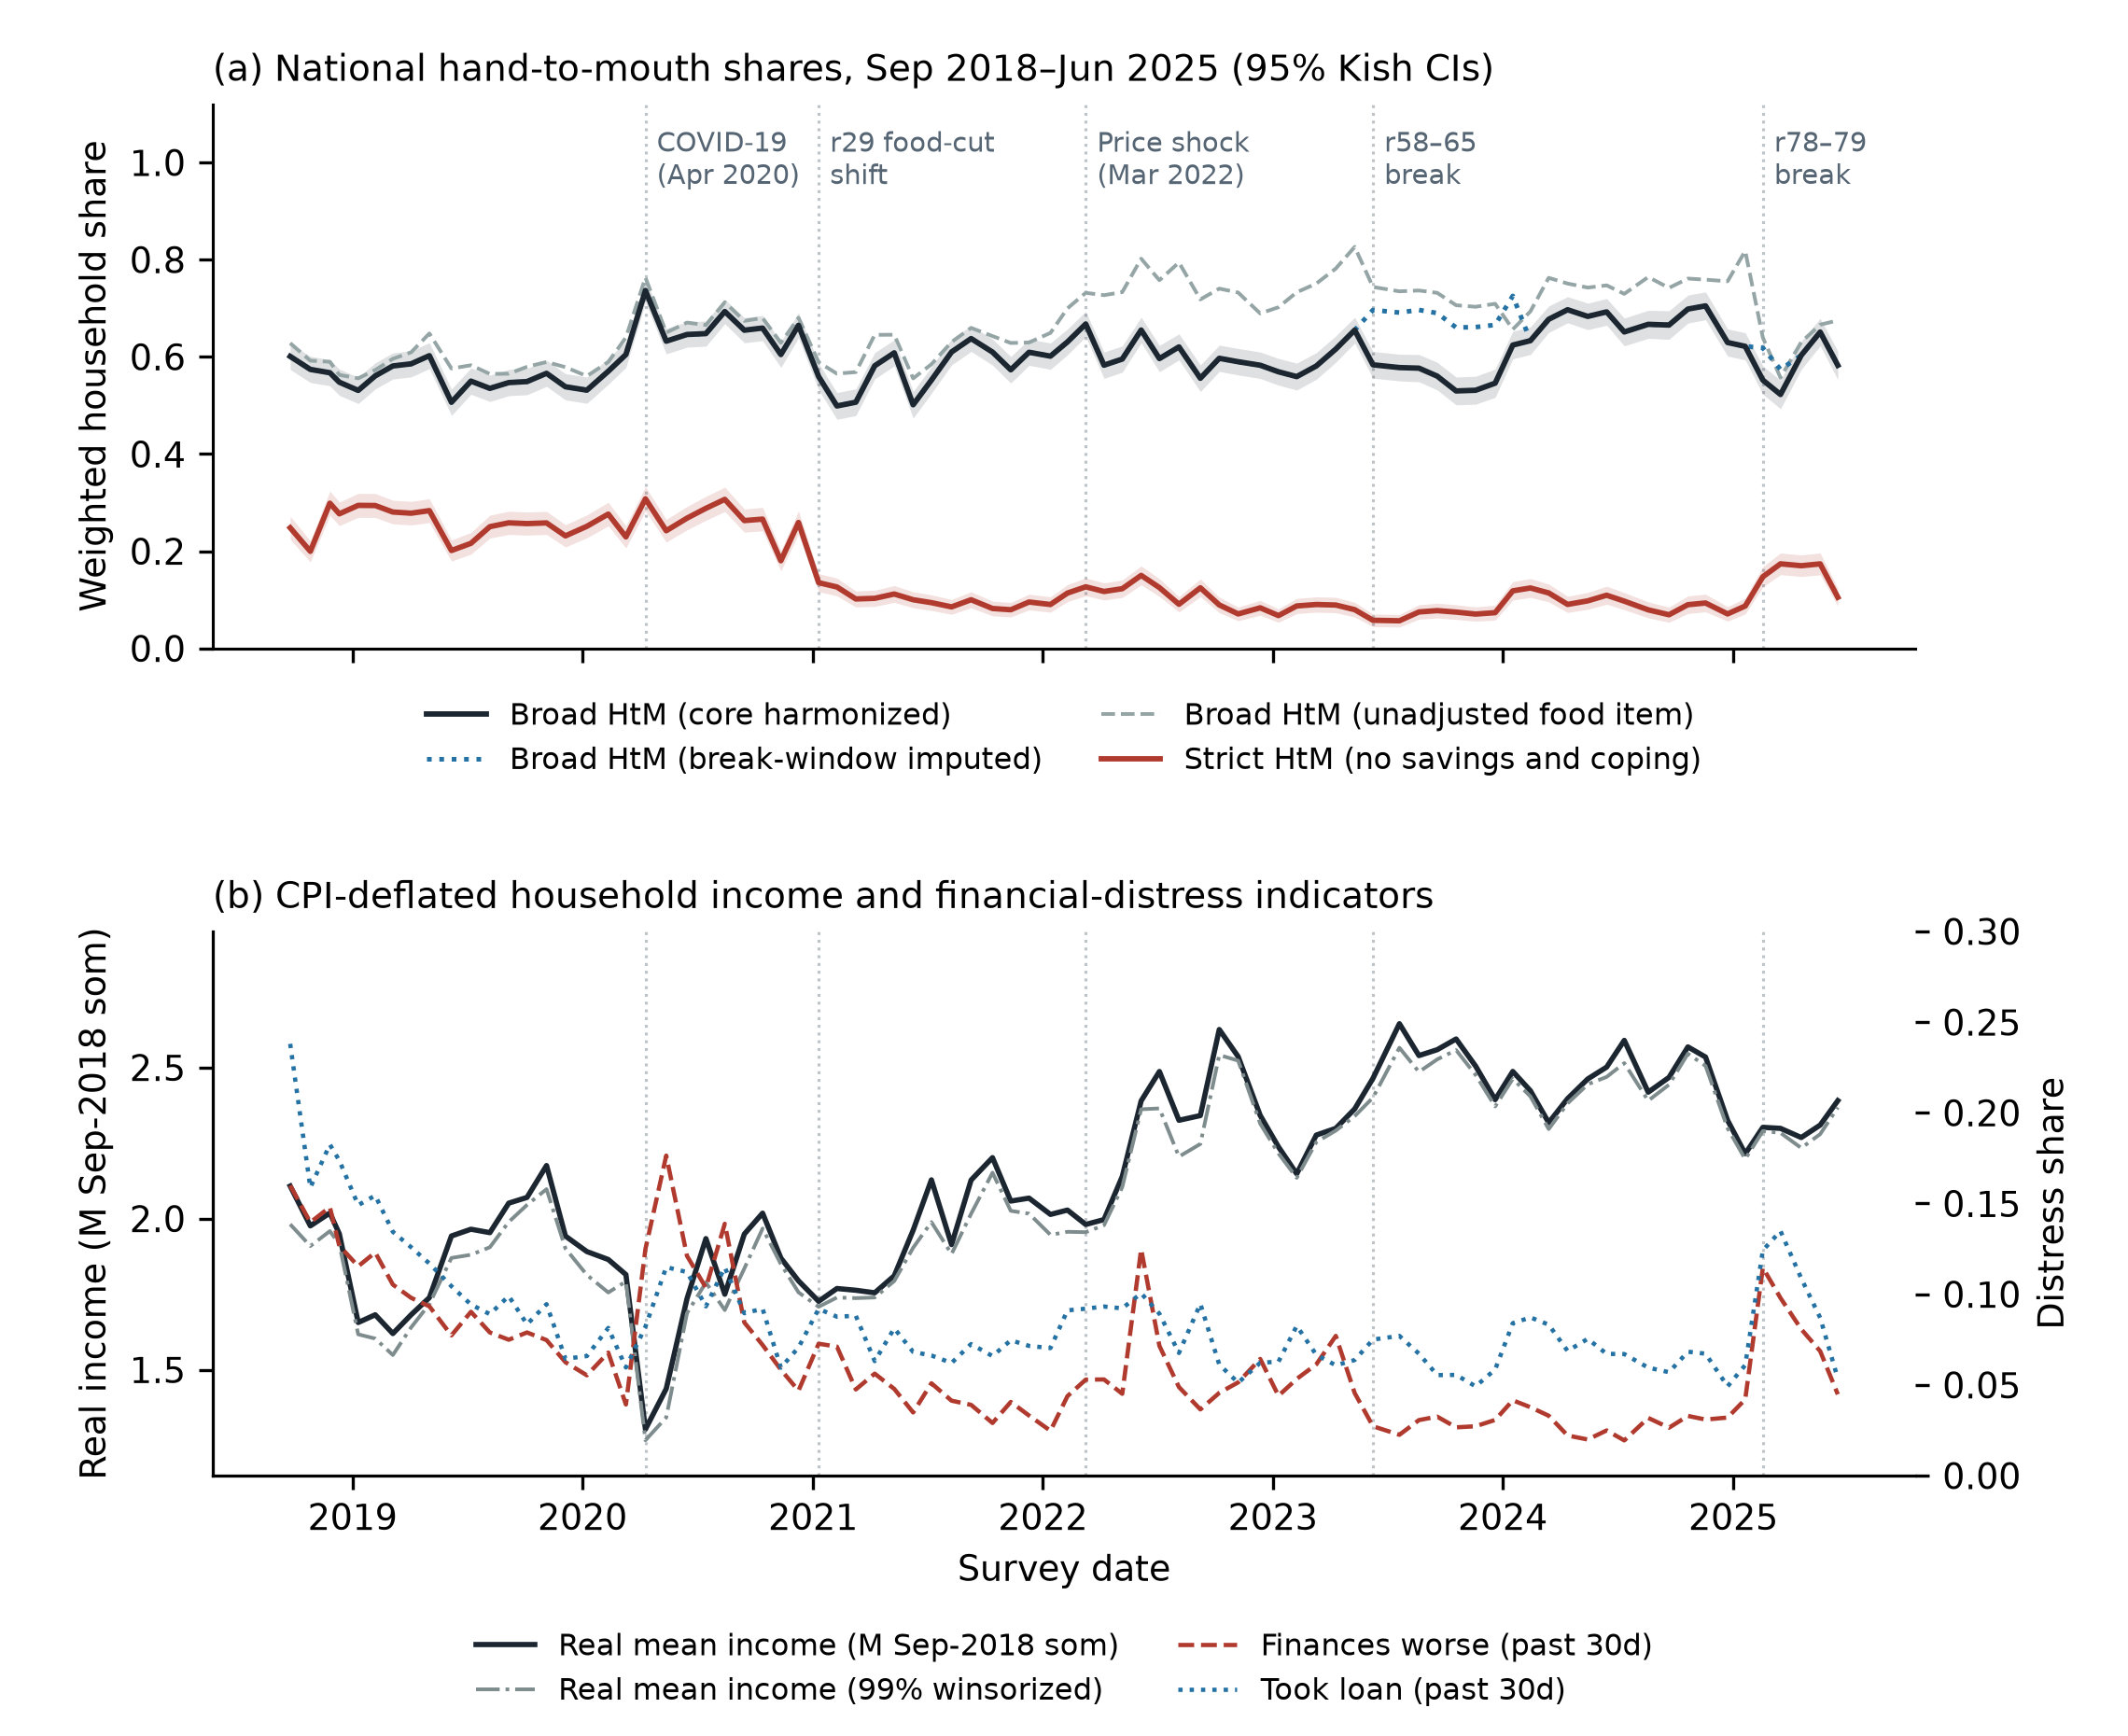
\includegraphics[width=0.96\linewidth]{../outputs/fig1_htm_dynamics.png}
\caption{National hand-to-mouth shares and real income dynamics in Uzbekistan, September 2018--June 2025. Panel (a) shows population-weighted core harmonized broad HtM and strict HtM with 95\% Kish bands, alongside break-window-imputed (dotted, active in r58--65 and r78--79) and unadjusted-food (dashed) broad HtM; vertical lines mark April 2020, the round-29 food-cut shift, the March 2022 price shock, and the r58--65 and r78--79 breaks. Panel (b) plots CPI-deflated monthly mean household income (raw and 99\% winsorized) alongside worsened finances and new loans.}
\label{fig:htm_dynamics}
\end{figure}

\begin{table}[tbp]
\centering
\caption{Selected L2CU rounds: sample sizes, weighted HtM shares, Kish SEs, and monthly income}
\label{tab:rounds}
\scriptsize
\setlength{\tabcolsep}{2.2pt}
\begin{tabular}{lccccccccc}
\toprule
Round (date) & $n$ & $n_{\text{eff}}$ & Broad (SE) & Strict (SE) & Broad$_{\text{win}}$ & Broad$_{\text{all}}$ & Broad$_{\text{unadj}}$ & Real $Y$ & Nom.\ $Y$ \\
\midrule
r01 (Sep 2018) & 1,504 & 1,281 & 0.601 (0.014) & 0.248 (0.012) & 0.601 & 0.601 & 0.628 & 2.11 & 2.11 \\
r19 (Mar 2020) & 1,522 & 1,303 & 0.605 (0.013) & 0.229 (0.012) & 0.605 & 0.623 & 0.640 & 1.81 & 2.27 \\
r20 (Apr 2020, COVID peak) & 1,521 & 1,302 & 0.737 (0.012) & 0.308 (0.013) & 0.737 & 0.755 & 0.763 & 1.30 & 1.66 \\
r30 (Feb 2021, trough) & 1,510 & 1,282 & 0.499 (0.014) & 0.126 (0.009) & 0.499 & 0.508 & 0.565 & 1.77 & 2.43 \\
r46 (Jun 2022, price shock) & 1,507 & 1,266 & 0.655 (0.013) & 0.150 (0.010) & 0.655 & 0.658 & 0.802 & 2.39 & 3.78 \\
r57 (May 2023, pre-break) & 1,488 & 1,247 & 0.655 (0.013) & 0.080 (0.008) & 0.655 & 0.655 & 0.826 & 2.36 & 4.09 \\
r58 (Jun 2023, break) & 1,486 & 1,244 & 0.584 (0.014) & 0.058 (0.007) & 0.696 & 0.697 & 0.744 & 2.46 & 4.25 \\
r61 (Sep 2023, break mid) & 1,439 & 1,173 & 0.560 (0.015) & 0.078 (0.008) & 0.690 & 0.691 & 0.732 & 2.56 & 4.49 \\
r75 (Nov 2024, pre-refresh) & 1,275 & 973 & 0.705 (0.015) & 0.093 (0.009) & 0.705 & 0.709 & 0.759 & 2.53 & 5.00 \\
r76 (Dec 2024, refresh) & 1,564 & 1,151 & 0.630 (0.014) & 0.071 (0.008) & 0.630 & 0.635 & 0.755 & 2.33 & 4.63 \\
r79 (Mar 2025, break/spike) & 1,492 & 1,110 & 0.522 (0.015) & 0.174 (0.011) & 0.574 & 0.576 & 0.557 & 2.30 & 4.68 \\
r82 (Jun 2025) & 1,463 & 1,089 & 0.582 (0.015) & 0.105 (0.009) & 0.582 & 0.588 & 0.675 & 2.39 & 4.96 \\
\midrule
Pooled (82 rounds) & 121,618 & -- & 0.599 (0.007) & 0.155 (0.005) & 0.613 & 0.636 & 0.672 & 2.13 & 3.32 \\
\bottomrule
\end{tabular}
\begin{flushleft}
\footnotesize\textit{Notes:} Population-weighted shares. Round parentheses report Kish SEs from Eq.~\eqref{eq:kish}; pooled parentheses report household-clustered SEs across 2,499 households from Eq.~\eqref{eq:clse}. Real $Y$ and Nom.\ $Y$ are monthly mean household incomes (including zero-income rounds) in millions of September-2018 som and nominal som \citep{StatUz2026CPI}.
\end{flushleft}
\end{table}

Once harmonized, the timeline tracks Uzbekistan's macroeconomic episodes closely. Before the pandemic (rounds 1--19), core and break-window-imputed broad HtM average 0.561 (all-round imputed 0.630) and strict HtM averages 0.257. During COVID-19 (rounds 20--29), broad HtM rises 9 percentage points to 0.650, jumping 13.2 percentage points in April 2020 alone (0.737 broad, 0.308 strict) as real mean income falls 28.2\% from 1.81M to 1.30M som. Every harmonized definition places April 2020 as the seven-year peak. During the 2021 recovery (rounds 30--42), broad HtM recedes to 0.579 and hits its sample low of 0.499 in February 2021. Removing the post-round-43 food artifact also eliminates an implausible 2023 spike: instead of jumping to 0.826 in May 2023 while real incomes were expanding on post-2022 remittance inflows, regional trade diversion, and wage and pension indexation, harmonized broad HtM averages 0.596 during the 2022--2023 price-shock window (rounds 43--55) and 0.620 in the late period (rounds 56--82; 0.660 window-imputed). Figure~\ref{fig:forensic_fig} compares these discontinuities against FIES food insecurity; the sharp initial drop in FIES from 0.51 to 0.35 across rounds 49--52 may partly reflect first-exposure panel conditioning.

\begin{figure}[tbp]
\centering
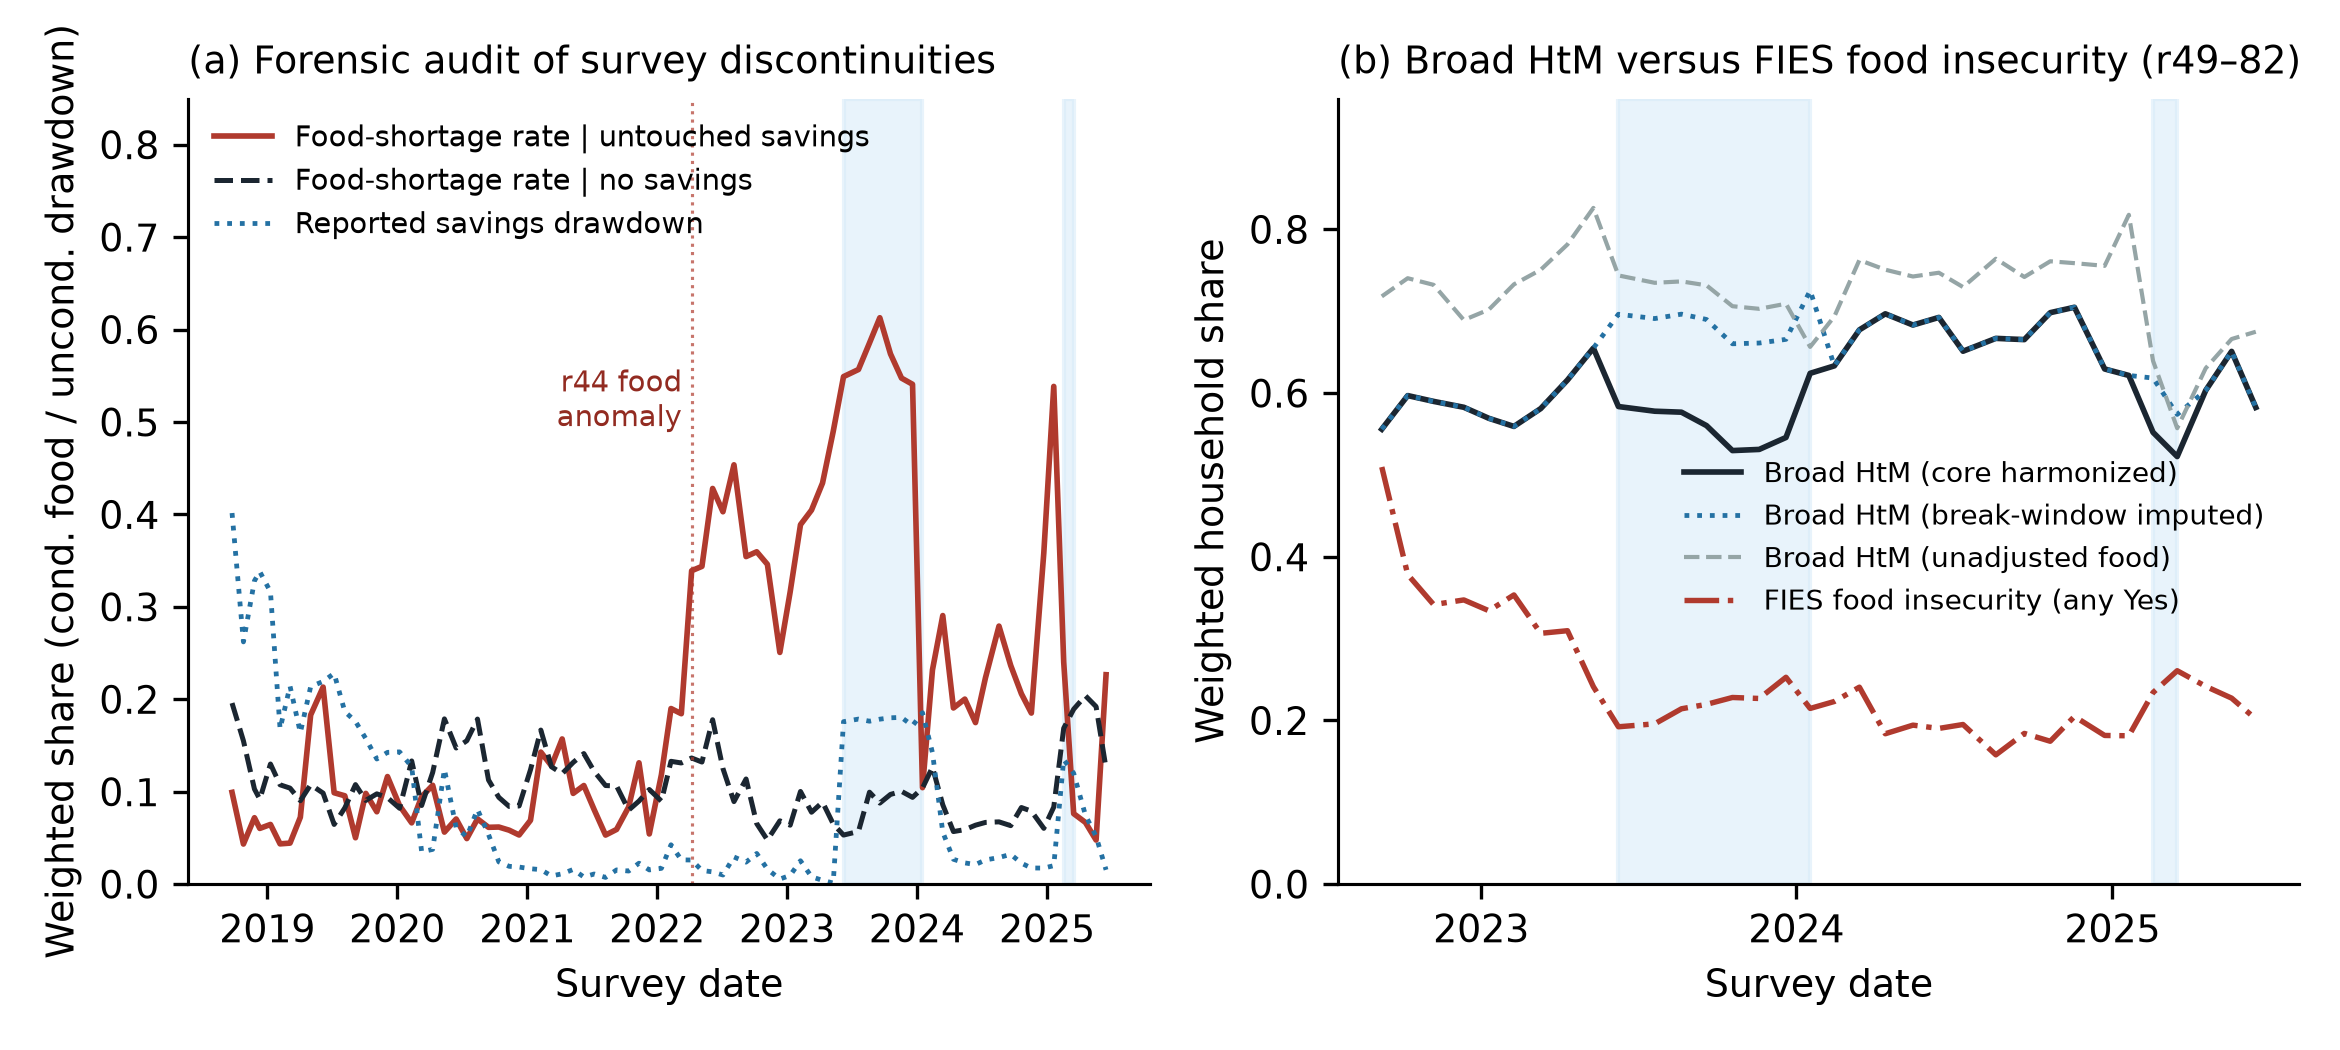
\includegraphics[width=0.96\linewidth]{../outputs/fig2_forensic_breaks.png}
\caption{Forensic audit of L2CU discontinuities and FIES comparison. Panel (a) plots conditional food-shortage rates among untouched savers versus no-savings households alongside unconditional reported savings drawdowns, highlighting the round-44 jump and shaded r58--65 and r78--79 breaks. Panel (b) compares FIES food insecurity (fielded from round 49) with core harmonized, break-window-imputed, and unadjusted-food broad HtM.}
\label{fig:forensic_fig}
\end{figure}

\section{Transitions, Income Risk, and Household Shock Exposure}\label{sec:dynamics}

\subsection{Three-state transition matrices and HMM misclassification correction}\label{sec:trans}

Table~\ref{tab:trans} summarizes monthly mobility across all 118,938 consecutive household-round pairs. Weighting shifts transition probabilities by at most 0.010 relative to unweighted counts, while household clustering widens standard errors by 1.5$\times$ to 2.6$\times$ over binomial formulas. Raw monthly retention rates in Panel A are 0.771 for savers ($S$), 0.732 for non-strict HtM ($M$), and 0.594 for strict HtM ($H$), implying stationary shares $\pi = (0.400, 0.448, 0.152)$ that match the pooled cross-section (window-imputed: $0.387, 0.459, 0.154$). Across the five subperiods in Panel B, stationary saver mass drops from 0.443 before COVID-19 to 0.362 during the pandemic and settles at 0.377 in rounds 56--82. Strict-HtM retention ($P_{H\to H}$) coincides at 0.677 in both the pre-COVID and COVID subperiods before stepping down to 0.454--0.522 after round 29 alongside the Q10 food-cut break.

Raw monthly transitions imply expected spells of only 2.5 to 4.4 months, raising a familiar concern from the labor-flows literature that phone-survey classification error inflates observed churn \citep{abowd1985effects}. Three-month sequences bear this out directly. Among households observed moving from $S_{t-1}$ to $M_t$, 44.6\% ($n = 8{,}543$) return to $S_{t+1}$ the very next month, compared with an unconditional $M \to S$ rate of 16.6\%. Similarly, 40.5\% of $M_{t-1} \to S_t$ movers ($n = 8{,}237$) revert to $M_{t+1}$, versus 19.0\% unconditionally.

To separate reporting noise from true persistence without confounding it with the round-29 food-cut break, Panel C estimates a population-weighted three-state Baum--Welch hidden-Markov model (HMM) with 50-draw household block-bootstrap standard errors on the post-round-29 sample (rounds 30--82, 2,134 contiguous runs). Once classification error is filtered out, underlying liquidity states are much more persistent: monthly retention rises to 0.968 (SE 0.001) for $S^*$, 0.976 (SE 0.002) for $M^*$, and 0.943 (SE 0.005) for $H^*$. Those probabilities imply expected spells of 31.2, 40.8, and 17.4 months, with exit from strict HtM moving primarily through $M^*$ rather than straight to $S^*$ ($A^*_{H^*\to M^*} = 0.039 > A^*_{H^*\to S^*} = 0.019$). The $3\times 3$ emission matrix $E$ shows clean accuracy for savers (86.9\%) and non-strict HtM (86.2\%), while 31.7\% of latent strict-HtM households are misclassified into $M$ and only 2.1\% into $S$ (accuracy 66.3\%).

Correcting for reporting noise puts the post-round-29 latent stationary broad-HtM share at 0.657 (SE 0.015; $\pi^* = [0.343, 0.553, 0.104]$). Three sensitivity checks in Panel C clarify initial-condition and break sensitivity. First, because round 30 coincides with the February 2021 trough ($\pi_0 = [0.521, 0.345, 0.134]$), post-2021 upward drift pulls asymptotic $\pi^* E = (0.351, 0.548, 0.101)$ above observed post-round-29 shares $(0.396, 0.504, 0.100)$ even though finite-horizon predicted shares $(0.408, 0.489, 0.103)$ track the data closely. Starting the HMM after the trough at round 36 (rounds 36--82, 2,103 runs) eliminates that drift: asymptotic $\pi^* E = (0.389, 0.508, 0.103)$ matches observed shares $(0.388, 0.513, 0.099)$ within 0.005, latent broad HtM sits at 0.606, and spell persistence remains equally long (36.7, 39.8, and 16.6 months). Second, re-estimating on break-window-imputed states in rounds 30--82 removes artificial r58--65 and r78--79 dips into $S$, raises log-likelihood by 545 points, improves saver accuracy to 88.6\%, and lifts latent broad HtM to 0.703 (SE 0.013; spells 28.5, 43.5, and 18.0 months). Third, re-estimating on the full Q10-excluded panel (rounds 1--82, 2,444 runs) yields spells of 27.7, 34.5, and 15.0 months and a latent broad-HtM share of 0.624 (SE 0.010). Because a homogeneous HMM abstracts from permanent mover--stayer heterogeneity, these durations are best read as upper bounds on single-household spells.

\begin{table}[tbp]
\centering
\caption{Monthly three-state HtM transitions, subperiod steady states, and weighted HMM misclassification model}
\label{tab:trans}
\scriptsize
\setlength{\tabcolsep}{2.0pt}
\resizebox{\linewidth}{!}{%
\begin{tabular}{lcccccc}
\toprule
\multicolumn{7}{l}{\textit{Panel A: Pooled weighted observed transitions (118,938 consecutive pairs; HH-clustered weighted SEs)}} \\
\midrule
From $\backslash$ To & Saver ($S$) & Non-strict HtM ($M$) & Strict HtM ($H$) & Pairs ($n$) & \multicolumn{2}{c}{HHs} \\
\midrule
Saver ($S$) & 0.771 (0.005) & 0.190 (0.004) & 0.039 (0.001) & 45,720 & \multicolumn{2}{c}{2,039} \\
Non-strict HtM ($M$) & 0.166 (0.004) & 0.732 (0.005) & 0.102 (0.003) & 54,365 & \multicolumn{2}{c}{2,209} \\
Strict HtM ($H$) & 0.115 (0.004) & 0.291 (0.007) & 0.594 (0.008) & 18,853 & \multicolumn{2}{c}{1,847} \\
\midrule
Steady state $\pi$ (wtd / uwtd) & 0.400 / 0.384 & 0.448 / 0.461 & 0.152 / 0.154 & \multicolumn{3}{c}{Spells: 4.4 / 3.7 / 2.5m} \\
\midrule
\multicolumn{7}{l}{\textit{Panel B: Regime-specific stationary distributions and strict-state persistence (weighted)}} \\
\midrule
Subperiod (transition rounds) & $\pi_S$ & $\pi_M$ & $\pi_H$ & \multicolumn{3}{c}{$P_{H \to H}$ (clustered SE)} \\
\midrule
Pre-COVID (r2--19) & 0.443 & 0.301 & 0.256 & \multicolumn{3}{c}{0.677 (0.010)} \\
COVID (r20--29) & 0.362 & 0.401 & 0.238 & \multicolumn{3}{c}{0.677 (0.010)} \\
2021 recovery (r30--42) & 0.408 & 0.492 & 0.100 & \multicolumn{3}{c}{0.522 (0.021)} \\
2022--23 price shock (r43--55) & 0.410 & 0.489 & 0.101 & \multicolumn{3}{c}{0.489 (0.016)} \\
Late period (r56--82) & 0.377 & 0.524 & 0.099 & \multicolumn{3}{c}{0.454 (0.021)} \\
\midrule
\multicolumn{7}{l}{\textit{Panel C: Weighted 3-state HMM on post-r29 regime (r30--82; 2,134 runs; 50-draw HH block-bootstrap SEs)}} \\
\midrule
Latent state & $A^*_{\cdot \to S^*}$ & $A^*_{\cdot \to M^*}$ & $A^*_{\cdot \to H^*}$ & $E_{\cdot \to S}$ & $E_{\cdot \to M}$ & $E_{\cdot \to H}$ \\
\midrule
$S^*$ (31.2m) & 0.968 (0.001) & 0.028 (0.001) & 0.004 (0.001) & 0.869 (0.006) & 0.112 (0.005) & 0.019 (0.001) \\
$M^*$ (40.8m) & 0.016 (0.001) & 0.976 (0.002) & 0.008 (0.001) & 0.091 (0.005) & 0.862 (0.005) & 0.047 (0.002) \\
$H^*$ (17.4m) & 0.019 (0.003) & 0.039 (0.004) & 0.943 (0.005) & 0.021 (0.004) & 0.317 (0.014) & 0.663 (0.015) \\
\midrule
Latent $\pi^*$ (SE) & 0.343 (0.015) & 0.553 (0.015) & 0.104 (0.005) & \multicolumn{3}{c}{Broad: 0.657 (0.015); $\pi_0$: 0.521/0.345/0.134} \\
Post-trough r36--82 $\pi^*$ & 0.394 & 0.499 & 0.108 & \multicolumn{3}{c}{Broad: 0.606; spells: 36.7/39.8/16.6m} \\
Break-win imp.\ r30--82 $\pi^*$ & 0.297 (0.013) & 0.591 (0.014) & 0.112 (0.008) & \multicolumn{3}{c}{Broad: 0.703 (0.013); spells: 28.5/43.5/18.0m} \\
Q10-excl.\ r1--82 $\pi^*$ & 0.376 (0.010) & 0.525 (0.010) & 0.099 (0.006) & \multicolumn{3}{c}{Broad: 0.624 (0.010); spells: 27.7/34.5/15.0m} \\
\bottomrule
\end{tabular}%
}
\begin{flushleft}
\footnotesize\textit{Notes:} Panel A covers all consecutive-round pairs under the core harmonized definition (max weighted vs.\ unweighted diff: 0.010). Panel B solves $\pi^{(r)} = \pi^{(r)} P^{(r)}$ per subperiod (unweighted $P_{H\to H}$ is 0.669 in pre-COVID and 0.670 in COVID; weighted coincides at 0.6769). Panel C estimates population-weighted Baum--Welch HMMs with full $3\times 3$ transition ($A^*$) and emission ($E$) matrices and 50-draw household block-bootstrap SEs (35 warm-started EM iterations per draw). Finite-horizon predicted observed shares $\bar{p}_{\text{pred}}$ are $(0.408, 0.489, 0.103)$ vs.\ observed $(0.396, 0.504, 0.100)$ in r30--82, and $(0.415, 0.476, 0.109)$ vs.\ observed $(0.412, 0.481, 0.108)$ in Q10-excluded r1--82; starting post-trough at r36--82 gives asymptotic $\pi^* E = (0.389, 0.508, 0.103)$ vs.\ observed $(0.388, 0.513, 0.099)$.
\end{flushleft}
\end{table}

\subsection{Income gaps, remittance and size robustness, and PPT decomposition}\label{sec:income}

Table~\ref{tab:income} compares real household incomes within each round and averages across all 82 waves. Strict-HtM households earn 34.2\% less than savers (weighted median log gap 0.418, level ratio 0.658), whereas non-strict HtM households earn 9.6\% less (median gap 0.101, mean gap 0.114). In the aggregate, savers account for 40.1\% of the population and earn 44.3\% of real income, while strict-HtM households make up 15.5\% of the population and earn 11.0\% of income. Strict-HtM families rely 2.6 times as heavily on social benefits (6.9\% versus 2.7\% of income) and report zero monthly cash income more often (6.5\% versus 4.7\%). Zero-income spells are short-lived: $P(Y_t = 0 \mid Y_{t-1} > 0) = 0.023$ ($n = 113{,}397$), and nearly half recover positive income the next month ($P(Y_t > 0 \mid Y_{t-1} = 0) = 0.480$, $n = 5{,}541$). Within-round income quintiles display a monotonic gradient, with broad HtM declining from 0.658 in the bottom quintile to 0.519 in the top quintile and strict HtM falling from 0.234 to 0.092.

Panel A checks whether these income shares are distorted by household size, extreme outliers, or omitted foreign remittances. Because weighted household size varies little across liquidity states ($S$: 5.88, $M$: 5.89, $H$: 5.66), switching to household-level weights ($w / n_{\text{hh}}$), per-capita income ($Y / n_{\text{hh}}$), or square-root equivalence scales ($Y / \sqrt{n_{\text{hh}}}$) leaves the saver income share between 0.443 and 0.444 and empirical $\text{AggMPC}_{\text{inc}}$ between 0.587 and 0.588. Winsorizing at the weighted within-round 99th percentile of positive real income (trimming 38 extreme reports above 50M nominal som) moves the saver share slightly to 0.438 ($\text{AggMPC}_{\text{inc}} = 0.592$). Adding individual-file foreign remittances (\texttt{mig\_living\_remittance\_amount} and \texttt{remittance\_hh\_amount}, converted to som at annual average Central Bank of Uzbekistan, CBU, rates) raises aggregate household income by 7.2\%. Because remittances represent nearly identical income shares across all three groups ($S$: 7.0\%, $M$: 7.5\%, $H$: 6.9\%), the saver income share moves by less than 0.001 (0.442 versus 0.443; $\text{AggMPC}_{\text{inc}} = 0.589$).

\begin{table}[tbp]
\centering
\caption{Within-round income gaps, robustness checks, and weighted PPT decomposition}
\label{tab:income}
\scriptsize
\setlength{\tabcolsep}{3.2pt}
\begin{tabular}{lcccc}
\toprule
\multicolumn{5}{l}{\textit{Panel A: Within-round real log-income gaps (82-round weighted average) and measurement checks}} \\
\midrule
Specification & $S - H$ gap & $S - M$ gap & Saver inc.\ share & Empirical $\text{AggMPC}_{\text{inc}}$ \\
\midrule
Baseline (person weights, median / mean gap) & 0.418 / 0.416 & 0.101 / 0.114 & 0.443 & 0.588 \\
Household weights ($w / n_{\text{hh}}$, median) & 0.469 & 0.109 & 0.444 & 0.587 \\
Per-capita real income ($Y / n_{\text{hh}}$, mean) & 0.358 & 0.118 & 0.444 & 0.587 \\
Square-root equivalized ($Y / \sqrt{n_{\text{hh}}}$, mean) & 0.387 & 0.116 & 0.443 & 0.588 \\
99\% within-round winsorized (mean gap) & 0.412 & 0.111 & 0.438 & 0.592 \\
Plus foreign remittances ($+7.2\%$ agg.\ $Y$, mean gap) & 0.428 & 0.112 & 0.442 & 0.589 \\
\bottomrule
\end{tabular}

\medskip
\begin{tabular}{lccc}
\toprule
\multicolumn{4}{l}{\textit{Panel B: Real income shares, sources, household size, and quintile HtM shares (weighted)}} \\
\midrule
Metric & Saver ($S$) & Non-strict HtM ($M$) & Strict HtM ($H$) \\
\midrule
Population share / Aggregate income share & 0.401 / 0.443 & 0.445 / 0.447 & 0.155 / 0.110 \\
Mean real monthly income (Sep-2018 som) & 2,355,874 & 2,141,332 & 1,513,926 \\
Mean household size / Zero-income share & 5.88 / 4.7\% & 5.89 / 3.5\% & 5.66 / 6.5\% \\
Wage / Self-employment / Pension share & 0.468 / 0.219 / 0.193 & 0.391 / 0.293 / 0.212 & 0.411 / 0.246 / 0.212 \\
Agriculture / Social benefits / Other share & 0.078 / 0.027 / 0.016 & 0.051 / 0.042 / 0.011 & 0.035 / 0.069 / 0.026 \\
Within-round quintiles (Q1 / Q3 / Q5) & \multicolumn{3}{c}{Broad: 0.658 / 0.612 / 0.519 \quad Strict: 0.234 / 0.145 / 0.092} \\
\bottomrule
\end{tabular}

\medskip
\setlength{\tabcolsep}{2.2pt}
\resizebox{\linewidth}{!}{%
\begin{tabular}{lcccccc}
\toprule
\multicolumn{7}{l}{\textit{Panel C: Minimum-distance weighted PPT decomposition (200-draw household block-bootstrap SEs)}} \\
\midrule
Specification & $\rho_z$ (SE) & Half-life (SE) & $\sigma_\alpha$ (SE) & $\sigma_\eta$ (SE) & $\sigma_\varepsilon$ (SE) & Shares ($\alpha / z / \varepsilon$) \\
\midrule
Lag 1--24 weighted (baseline) & 0.923 (0.008) & 8.7m (1.0) & 0.574 (0.013) & 0.141 (0.005) & 0.404 (0.006) & 52.6 / 21.3 / 26.1\% \\
Lag 1--12 weighted (truncated) & 0.772 (0.015) & 2.7m (0.2) & 0.622 (0.011) & 0.196 (0.006) & 0.380 (0.006) & 61.7 / 15.2 / 23.1\% \\
Lag 1--48 weighted (long horizon) & 0.959 (0.005) & 16.6m (2.1) & 0.525 (0.019) & 0.120 (0.004) & 0.413 (0.006) & 43.9 / 28.8 / 27.3\% \\
Lag 1--24 net of $\mu_s$ (microsim) & 0.928 (0.008) & 9.3m (1.1) & 0.551 (0.015) & 0.138 (0.004) & 0.412 (0.005) & 49.8 / 22.4 / 27.8\% \\
Lag 1--24 never-ag ($G=1{,}373$) & 0.924 (0.011) & 8.8m (1.4) & 0.628 (0.022) & 0.139 (0.007) & 0.337 (0.009) & 61.7 / 20.6 / 17.7\% \\
Lag 1--24 ever-ag ($G=1{,}097$) & 0.921 (0.011) & 8.4m (1.2) & 0.539 (0.017) & 0.140 (0.006) & 0.445 (0.008) & 47.1 / 20.8 / 32.1\% \\
\bottomrule
\end{tabular}%
}
\begin{flushleft}
\footnotesize\textit{Notes:} Panel A evaluates empirical $\text{AggMPC}_{\text{inc}} = \sum_s \omega_s m_s$ at $(m_S, m_M, m_H) = (0.07, 1.00, 1.00)$. The 99\% winsorized row caps real income at the weighted within-round 99th percentile of positive incomes consistently across gaps and shares. The remittance row converts individual-file foreign remittances (USD/RUB/KZT/UZS) at annual average Central Bank of Uzbekistan (CBU) rates and adds them to $Y_{it}$. Panel C fits Eq.~\eqref{eq:autocov} via equally weighted minimum distance on round-demeaned positive real log incomes ($n = 115{,}909$ obs., 2,470 households); RMSE is 0.0054 (lag 1--24), 0.0009 (lag 1--12), 0.0063 (lag 1--48), 0.0053 (net of $\mu_s$), 0.0035 (never-agricultural), and 0.0070 (ever-agricultural).
\end{flushleft}
\end{table}

To separate permanent cross-household differences from persistent income shocks and monthly reporting noise, we fit a standard permanent-persistent-transitory (PPT) process by equally weighted minimum distance to round-demeaned positive real log income $r_{it} = \ln Y_{it} - \overline{\ln Y}_t$ ($n = 115{,}909$ observations across 2,470 households):
\begin{equation}\label{eq:ppt}
r_{it} = \alpha_i + z_{it} + \varepsilon_{it}, \qquad z_{it} = \rho_z z_{i,t-1} + \eta_{it},
\end{equation}
which implies the theoretical autocovariance profile
\begin{equation}\label{eq:autocov}
\text{Cov}(r_{it}, r_{i,t+k}) = \begin{cases}
\sigma_\alpha^2 + \sigma_z^2 + \sigma_\varepsilon^2 & \text{if } k = 0, \\
\sigma_\alpha^2 + \rho_z^k \sigma_z^2 & \text{if } k \ge 1,
\end{cases}
\end{equation}
with $\sigma_z^2 = \sigma_\eta^2 / (1 - \rho_z^2)$ \citep{blundell2008consumption,guvenen2009empirical}. Weighted autocovariances decline from 0.627 at $k = 0$ to 0.461 at $k = 1$, 0.391 at $k = 12$, 0.348 at $k = 24$, and 0.294 at $k = 48$. Matching lags 1 through 24 gives $\rho_z = 0.923$ (bootstrap SE 0.008; half-life 8.7 months), attributing 52.6\% of log-income variance to permanent heterogeneity, 21.3\% to persistent risk, and 26.1\% to transitory or measurement noise (after netting out state means $\mu_{s_{it}}$ for the microsimulation, $\rho_z = 0.928$).

Because round fixed effects remove the national seasonal mean but not household-level harvest cycles, Panel C also splits the panel into households that never report agricultural cash income ($G = 1{,}373$) and those that ever do ($G = 1{,}097$). Agricultural households display a clear 12-month seasonal rebound in their autocovariances at lags 12 and 36 (rising from 0.352 at lag 11 to 0.353 at lag 12, and from 0.282 at lag 30 to 0.287 at lag 36), along with higher transitory volatility ($\sigma_\varepsilon = 0.445$ versus $0.337$) and higher RMSE (0.0070). Non-agricultural households exhibit smooth monotonic decay and half the RMSE (0.0035). Despite that seasonal contrast, the persistent-shock parameters are virtually identical across both groups: $\rho_z = 0.924$ and $\sigma_\eta = 0.139$ for non-agricultural households versus $\rho_z = 0.921$ and $\sigma_\eta = 0.140$ for agricultural households. Since autocovariances continue edging down between lags 24 and 48 (raising lag-48 $\hat{\rho}_z$ to 0.959), multi-year dynamics may also include a slower random-walk component or late-panel attrition; we adopt the lag-24 estimate $\rho_z = 0.928$ as our monthly calibration.

\subsection{Behavioral validation of \texorpdfstring{$M_1$}{M1}, job-loss exposure, and institutional checks}\label{sec:exposure}

Because 92.6\% of non-strict HtM households ($M_1$, 41.2\% of the population) report having no savings without taking any active coping measure, it is important to check whether $M_1$ reflects genuine buffer vulnerability rather than classification noise indistinguishable from Savers ($S$). Table~\ref{tab:m1val} compares $S$, $M_1$, and $H$ across independent indicators in L2CU. On every cross-sectional marker in Panel A, $M_1$ sits well above Savers while remaining well below acute strict-HtM distress: relative to $S$, $M_1$ households experience 2.03$\times$ higher FIES food insecurity (0.258 versus 0.127), 2.70$\times$ higher utility arrears (4.2\% versus 1.6\%), 1.49$\times$ higher delayed or unaffordable medical care (9.2\% versus 6.2\%), 1.90$\times$ more frequent reports of bad local economic conditions (12.4\% versus 6.6\%), and only 0.41$\times$ the rate of realized past-30-day saving (1.9\% versus 4.6\%; all $p < 0.001$).

Panel B compares dynamic shock responses in weighted Round-FE regressions. When a household member loses work, $M_1$ households raise emergency borrowing by $+13.1$ percentage points (SE 1.8 pp) versus $+7.7$ percentage points (SE 1.7 pp) for Savers, a statistically significant gap of $+5.4$ pp ($t = 2.17$, $p = 0.03$). Post-job-loss jumps in worsened finances ($+15.5$ versus $+12.8$ pp, $t = 1.02$) and FIES food insecurity ($+16.1$ versus $+11.1$ pp, $t = 0.61$) are also larger for $M_1$, though the differences against $S$ are not statistically distinct. Similarly, on weekly flour spending ($n = 28{,}092$ consecutive positive pairs including $M_2$; $n = 27{,}170$ across $S, M_1, H$ in Table~\ref{tab:m1val}), the income elasticity for $M_1$ ($+0.027$, SE 0.011, $p = 0.01$) is more than twice that of Savers ($+0.012$, SE 0.009), yet the difference between the two slopes is imprecise ($t = 1.09$), and combined bread-and-flour elasticities are nearly flat across groups ($+0.021$ for $S$, $+0.019$ for $M_1$). Taken together, Panel A and the emergency-borrowing response confirm that $M_1$ households carry thinner liquid buffers than Savers while sitting clearly below acute strict-HtM distress. Section~\ref{sec:model} therefore evaluates all main results across a wide range $m_M \in [0.50, 1.00]$.

\begin{table}[tbp]
\centering
\caption{Behavioral validation of pure no-savings ($M_1$) versus Savers and Strict HtM}
\label{tab:m1val}
\scriptsize
\setlength{\tabcolsep}{3.6pt}
\begin{tabular}{lcccc}
\toprule
\multicolumn{5}{l}{\textit{Panel A: Independent welfare and saving markers (weighted means, HH-clustered SEs)}} \\
\midrule
Indicator & Saver ($S$) & Pure no-sav ($M_1$) & Strict HtM ($H$) & Ratio $M_1 / S$ \\
\midrule
FIES food insecurity (r49--82) & 0.127 (0.005) & 0.258 (0.010) & 0.640 (0.020) & 2.03$\times$ \\
Utility payment arrears (past 30d) & 0.016 (0.001) & 0.042 (0.003) & 0.254 (0.009) & 2.70$\times$ \\
Delayed/unaffordable medical care (30d) & 0.062 (0.002) & 0.092 (0.005) & 0.282 (0.009) & 1.49$\times$ \\
Bad local economic conditions & 0.066 (0.003) & 0.124 (0.006) & 0.245 (0.012) & 1.90$\times$ \\
Realized saving in past 30 days & 0.046 (0.002) & 0.019 (0.002) & 0.008 (0.001) & 0.41$\times$ \\
\midrule
\multicolumn{5}{l}{\textit{Panel B: Dynamic shock responses by lagged state $s_{t-1}$ (weighted Round-FE, clustered SEs)}} \\
\midrule
Outcome / Regression & Lag $S$ & Lag $M_1$ & Lag $H$ & $M_1 - S$ ($t$-stat) \\
\midrule
Job loss $\to \Delta P(\text{Loan}_t)$ & $+0.077$ (0.017) & $+0.131$ (0.018) & $+0.181$ (0.024) & $+0.054$ (2.17) \\
Job loss $\to \Delta P(\text{Fin.\ worse}_t)$ & $+0.128$ (0.018) & $+0.155$ (0.019) & $+0.202$ (0.022) & $+0.027$ (1.02) \\
Job loss $\to \Delta P(\text{FIES}_t)$ & $+0.111$ (0.064) & $+0.161$ (0.052) & $+0.183$ (0.087) & $+0.050$ (0.61) \\
Flour elasticity $\Delta \ln c_{it}$ on $\Delta r_{it}$ & $+0.012$ (0.009) & $+0.027$ (0.011) & $+0.029$ (0.016) & $+0.015$ (1.09) \\
\bottomrule
\end{tabular}
\begin{flushleft}
\footnotesize\textit{Notes:} Panel A separates $M_1$ (no savings, no active coping; 92.6\% of $M$) from $S$ and $H$ across all 82 rounds (FIES r49--82); all $M_1$ vs.\ $S$ differences in Panel A have $p < 0.001$. Panel B estimates weighted Round-FE regressions with household-clustered SEs by lagged state; the final column reports the difference $M_1 - S$ and its conservative two-sample $t$-statistic (joint household-clustered covariance across overlapping households yields $t = 2.26$ for loans). Flour-elasticity sample sizes are $n_S = 10{,}903$, $n_{M_1} = 11{,}934$, $n_H = 4{,}333$ (bread elasticities are $+0.023$, $+0.027$, and $+0.016$; combined bread+flour elasticities are $+0.021$, $+0.019$, and $+0.025$, none statistically distinct across states).
\end{flushleft}
\end{table}

We next examine who absorbs labor-market shocks. Tracing the sample from all 121,618 household-rounds: 118,938 consecutive pairs enter Table~\ref{tab:trans}, 118,907 household-rounds merge to the individual labor file, and 116,249 consecutive linked pairs ($44{,}382$ in $S$, $53{,}498$ in $M$, and $18{,}369$ in $H$) enter Table~\ref{tab:workloss}. Regressing monthly HtM transitions directly on noisy log-income changes $\Delta r_{it}$ produces near-zero slopes ($-0.002$, SE 0.004 for $S_{t-1} \to B_t$) because 26.1\% transitory noise attenuates month-to-month first differences. Using an observed labor shock, whether any household member lost work in round $t$, avoids this attenuation. Across the panel, 2,189 job-loss events occur; weighted monthly incidence averages 3.34\% pre-COVID (r1--19), 6.12\% during COVID (r20--29), and 0.62\% post-COVID (r30--82), tapering smoothly across rounds 29 to 32 (3.95\%, 1.89\%, 1.16\%, and 0.69\%) rather than breaking abruptly at round 29 like Q10. Because 79.1\% of events occur in 2018--2020, every specification includes round fixed effects.

\begin{table}[tbp]
\centering
\caption{Household job-loss exposure (lags $t-1$ to $t-3$), switching effects, and event-study dynamics}
\label{tab:workloss}
\scriptsize
\setlength{\tabcolsep}{1.4pt}
\begin{tabular}{lcccccccc}
\toprule
\multicolumn{9}{l}{\textit{Panel A: Primary weighted Round-FE job-loss effects by lagged state $s_{t-1}$ (HH-clustered SEs)}} \\
\midrule
State & WL rate & $\Delta \ln Y$ & $\Delta P(+\!\to\!0)$ & Total & $\Delta P(B_t)$ & $\Delta P(H_t)$ & HH+Rd FE & Pre-trend \\
$s_{t-1}$ & (wtd) & (SE) & (SE) & $\% \Delta Y$ & (SE) & (SE) & $B$ / $H$ & $\Delta r_{t-1}$ (SE) \\
\midrule
$S_{t-1}$ & 0.0107 & $-0.197$ (0.039) & $+0.048$ (0.016) & $-21.8\%$ & $+0.229$ (0.026) & $+0.203$ (0.023) & $+0.146$/$+0.169$ & $-0.104$ (0.036) \\
$M_{t-1}$ & 0.0152 & $-0.265$ (0.033) & $+0.052$ (0.013) & $-27.3\%$ & $+0.032$ (0.016) & $+0.160$ (0.019) & $+0.098$/$+0.127$ & $+0.005$ (0.027) \\
$H_{t-1}$ & 0.0524 & $-0.247$ (0.028) & $+0.078$ (0.015) & $-27.9\%$ & $+0.083$ (0.008) & $+0.177$ (0.016) & $+0.072$/$+0.117$ & $-0.067$ (0.027) \\
\bottomrule
\end{tabular}

\medskip
\begin{tabular}{lccccc}
\toprule
\multicolumn{6}{l}{\textit{Panel B: Lagged exposure robustness ($t-1, t-2, t-3$; raw ratios and Round-FE gaps vs.\ $S$)}} \\
\midrule
Lag horizon & Full raw $H/S$ & Rd-FE $M-S$ (SE) & Rd-FE $H-S$ (SE) & r30--82 $H/S$ & r30--82 Rd-FE $H-S$ \\
\midrule
Lag $t-1$ & 4.91$\times$ & $+0.0069$ (0.0009) & $+0.0337$ (0.0027) & 7.23$\times$ & $+0.0170$ (0.0025) \\
Lag $t-2$ & 4.13$\times$ & $+0.0058$ (0.0009) & $+0.0300$ (0.0027) & 5.92$\times$ & $+0.0138$ (0.0024) \\
Lag $t-3$ & 4.00$\times$ & $+0.0036$ (0.0009) & $+0.0300$ (0.0027) & 4.96$\times$ & $+0.0114$ (0.0021) \\
\bottomrule
\end{tabular}

\medskip
\setlength{\tabcolsep}{4.0pt}
\begin{tabular}{lcccccccc}
\toprule
\multicolumn{9}{l}{\textit{Panel C: Job-loss event study on real log income ($\ln Y_{t+h} - \ln Y_{t-2}$, weighted Round-FE, clustered SEs)}} \\
\midrule
Horizon $h$ & $h=-3$ & $h=-1$ & $h=0$ & $h=+1$ & $h=+2$ & $h=+3$ & $h=+6$ & $h=+12$ \\
\midrule
$\hat{\beta}_h$ & $-0.005$ & $-0.051$ & $-0.274$ & $-0.181$ & $-0.159$ & $-0.136$ & $-0.071$ & $-0.071$ \\
(Clustered SE) & (0.015) & (0.015) & (0.019) & (0.019) & (0.019) & (0.019) & (0.020) & (0.022) \\
\bottomrule
\end{tabular}
\begin{flushleft}
\footnotesize\textit{Notes:} Consecutive linked pairs ($n = 116{,}249$; positive pairs for $\Delta \ln Y$: $108{,}272$). ``WL rate'' is the weighted monthly household job-loss incidence. Total $\% \Delta Y = (1 - \Delta P_{\text{zero}})\exp(\hat{\beta}_{\Delta \ln Y}) - 1$. In Panel A, HH+Rd FE $\Delta \ln Y$ slopes are $-0.204$ ($S$), $-0.277$ ($M$), and $-0.269$ ($H$), all $p < 0.001$; for $H_{t-1}$, $\Delta P(H_t)$ reflects elevated strict-HtM persistence rather than entry. Panel B tests job-loss exposure at $t-1, t-2, t-3$ both raw and with Round FE (all $H-S$ gaps $t > 5.3$ post-COVID and $t > 11.0$ full sample). Panel C traces real log-income paths relative to $t-2$ ($n = 83{,}465$ to $105{,}961$).
\end{flushleft}
\end{table}

Table~\ref{tab:workloss} shows that job loss concentrates heavily among households that are already financially exposed. At lag $t-1$, strict-HtM households lose work at 5.24\% per month versus 1.07\% for savers, a 4.91$\times$ ratio with a Round-FE gap of $+3.37$ percentage points ($t = 12.6$). Neither one-month anticipation nor 2018--2020 time composition drives this gradient: lagging liquidity status to $t-2$ or $t-3$ leaves the full-sample ratio at 4.00$\times$--4.13$\times$ (Round-FE gap $+3.00$ pp, $t > 11.0$) and the post-COVID ratio (rounds 30--82) at 4.96$\times$--5.92$\times$ ($t > 5.3$).

Combining intensive log-income drops with transitions into zero income produces total real income losses upon job loss of $-21.8\%$ for savers, $-27.3\%$ for non-strict HtM, and $-27.9\%$ for strict HtM. Job loss also drives state switching: affected savers are 22.9 percentage points more likely to enter broad HtM ($+20.3$ pp into $H$ and $+2.6$ pp into $M$; $+14.6$ pp with household fixed effects), affected $M$ households enter strict HtM at a $+16.0$ pp higher rate ($+12.7$ pp HH-FE), and affected $H$ households remain in strict HtM at a $+17.7$ pp higher rate ($+11.7$ pp HH-FE). Adding household fixed effects absorbs each household's baseline propensity to cycle between $M$ and $S$, which lifts the broad-HtM retention effect for $M_{t-1}$ from $+0.032$ to $+0.098$. Panel A also records statistically significant negative one-month pre-trends $\Delta r_{t-1}$ for savers ($-0.104$, SE 0.036) and strict-HtM households ($-0.067$, SE 0.027), mirroring the pooled $-0.051$ dip at $h = -1$ in Panel C (with a flat pre-trend of $-0.005$ at $h = -3$) and pointing to pre-separation hours cuts or wage arrears before formal job loss. On impact, pooled real log income falls $-0.274$ and retains an earnings scar of $-0.071$ (SE 0.022) twelve months later.

We read Table~\ref{tab:workloss} as descriptive conditional dynamics rather than pure causal identification, and the contrast with broader aggregate fluctuations is instructive. In non-COVID months, regressing household log-income growth $\Delta \ln Y_{it}$ on aggregate growth $\Delta \ln \bar{Y}_t$ yields modestly steeper cyclicality for strict HtM ($1.19$, SE $0.09$) than for savers ($1.01$, SE $0.06$, at lag $t-1$; $1.12$ versus $0.99$ at lag $t-2$). By contrast, the April 2020 lockdown shut down formal and informal earners alike, cutting real mean income broadly across every pre-COVID group ($-31.8\%$ in $S$, $-24.6\%$ in $M$, and $-26.7\%$ in $H$ by round-19 state). Regressive incidence thus appears primarily in labor-displacement downturns, whereas universal lockdowns hit all liquidity groups similarly.

Two institutional facts from L2CU's supplementary modules complete the empirical picture:
\begin{itemize}
\item \textit{Remittances fund food consumption and illiquid housing investment.} Roughly 6.1\% of linked household-rounds ($n = 7{,}295$) report an active migrant sending money home \citep{kakhkharov2017transaction,seitz2019migration,abduvaliev2020impact,kakhkharov2021south}. Across 8,096 primary-use reports, half go to food (50.0\%) and more than a quarter go to housing repair or construction (27.1\%), while only 3.4\% enter liquid financial savings. In Central Asia, residential construction and home improvement (\textit{uy qurish}) act as a primary vehicle for illiquid household wealth accumulation rather than nondurable spending, consistent with low formal deposit usage. Because very few remittance recipients suffer job loss in a given month ($n = 12$ in $S$, $18$ in $M$, and $22$ in $H$), exact within-round permutation tests (2,000 draws) on cross-border shock buffering remain statistically underpowered ($p = 0.307, 0.146, 0.927$).
\item \textit{Payment cards are widespread, yet savings remain in cash at home.} Among the 3,429 household-rounds (2.8\%) reporting realized past-30-day saving (Catalog 6412 saving module, Appendix~\ref{app:dict}; 65.4\% in $S$, 30.9\% in $M$, 3.8\% in $H$; median saving-to-income ratio 0.30), 94.8\% ($3{,}250/3{,}429$) keep those savings as cash at home while only 3.1\% ($107/3{,}429$) use bank deposits. This ratio is close to Uzbekistan's 2.6\% adult formal-saving rate in Global Findex 2021 \citep{demirguckunt2022findex}, even though survey denominators differ. Over the same period, weighted bank-card ownership rises from 65.8\% in round 40 to 85.1\% in round 82, remaining flat across liquidity states ($S$: 77.3\%, $M$: 76.8\%, $H$: 76.2\% pooled), with at least 95\% of cardholders actively receiving transfers, making purchases, and withdrawing cash. Bank cards in Uzbekistan function as payment rails rather than formal savings accounts, precluding a balance-sheet wealthy-HtM test \citep{kaplan2014wealthy}. Affirmative realized-saving reports also decline from 13.6\% in round 1 to 1.6\% across rounds 75--82, suggesting late-panel respondent fatigue alongside tighter household budgets.
\end{itemize}

\section{IBC-Consistent Three-State Markov-TANK Microsimulation}\label{sec:model}

\subsection{Model specification and smoothed buffer-rebuilding IBC}\label{sec:modelspec}

To map these household moments into dynamic spending paths, we run a partial-equilibrium three-state microsimulation of $N = 40{,}000$ households over 161 months: a 30-month burn-in, an aggregate shock at $t^* = 40$, and 120 post-shock horizons ($h = 0, \dots, 120$). Every counterfactual uses identical common random numbers (CRN, seed 12345). Prices, wages, and interest rates are fixed, so the exercise offers partial-equilibrium accounting disciplined directly by L2CU moments.

Each household occupies state $s_{it} \in \{S, M, H\}$ evolving via the empirical transition matrix $P$ (or the weighted HMM kernel $A^*$), draws permanent heterogeneity $\alpha_i \sim \mathcal{N}(0, \sigma_\alpha^2)$, and receives persistent income $z_{it} = \rho_z z_{i,t-1} + \eta_{it} + \delta_{i,t}$ parameterized by our net-of-$\mu_s$ lag-24 PPT estimates $(\rho_z, \sigma_\alpha, \sigma_\eta) = (0.928, 0.551, 0.138)$. Baseline real income is
\begin{equation}\label{eq:income_sim}
y_{it}^{\text{base}} = \exp\!\left(\mu_{s_{it}^{\text{base}}} + \alpha_i + z_{it}^{\text{base}}\right),
\end{equation}
anchored to $\mu = (14.416, 14.302, 14.000)$ so baseline income matches saver mean real log income and exact within-round mean gaps ($S - M = 0.114$, $S - H = 0.416$).

A static spending rule ($c_{it}^{\text{shock}} = y_{it}^{\text{base}} + m_s \Delta y_{it}$) violates the household intertemporal budget constraint whenever $m_s < 1$. At the opposite extreme, forcing a household switching from $S$ into $M$ or $H$ to absorb its entire accumulated liquid-asset deviation $(1+r)\Delta a_{i,t-1}$ in one month behaves like an abrupt 100\% credit recall, triggering 148 post-shock zero-consumption floor hits under raw noisy transitions. Our baseline instead uses a smoothed buffer-rebuilding rule at monthly real return $r = 0.0025$ (3\% annualized, paired with an $r = 0$ cash-at-home check). Tracking each household's asset deviation $\Delta a_{it}$ from baseline ($\Delta a_{i,t^*-1} = 0$), current income shocks are spent at the current state's MPC $m_{s_{it}^{\text{shock}}}$, while prior buffer drawdowns are rebuilt gradually at rate $\delta_a = m_S$:
\begin{equation}\label{eq:ibc_rule}
\begin{aligned}
\Delta c_{it} &= m_{s_{it}^{\text{shock}}}\Delta y_{it} + \delta_a (1 + r)\Delta a_{i,t-1}, \qquad
\Delta a_{it} = (1 + r)\Delta a_{i,t-1} + \Delta y_{it} - \Delta c_{it}, \\
c_{it}^{\text{shock}} &= \max\!\left(0,\; y_{it}^{\text{base}} + \Delta c_{it}\right).
\end{aligned}
\end{equation}
On impact ($h = 0$), $\Delta c_{i,t^*} = m_{s_{it^*}}\Delta y_{i,t^*}$. For $h \ge 1$, the decay factor $(1 - \delta_a)(1 + r) = 0.932 < 1$ ensures asymptotic present-value closure (a 120-month PV ratio of 1.000 at $m_S = 0.07$ and 0.982 at $m_S = 0.03$) with zero floor hits across all 4.84 million post-shock household-months. Because smoothed rebuilding allows newly constrained households to unwind negative asset deviations gradually, Table~\ref{tab:counterfactuals} also reports the strict no-borrowing \textit{callable-debt clawback} variant ($\delta_a = m_{s_{it}^{\text{shock}}}$) under both $P$ and the HMM kernel $A^*$, alongside two forward-looking benchmarks: a \textit{forward-looking buffer-stock iMPC rule} with $m_S^{\text{FL}} = m_S / [1 - (1 - m_S)\rho_z/(1+r)] = 0.503$ \citep{auclert2024intertemporal} ($\Delta c_{it} = m_S^{\text{FL}}\Delta y_{it} + m_S(1+r)\Delta a_{i,t-1}$ for savers, which preserves exact PV closure), and a \textit{fixed-status infinite-horizon PIH benchmark} ($P = I$) with saver rule $\Delta c_{it} = \frac{r}{1+r}\bigl[(1+r)\Delta a_{i,t-1} + \Delta y_{it}\frac{1+r}{1+r-\rho_z}\bigr]$ and impact MPC $m_S^{\text{PIH}} = r / (1 + r - \rho_z) = 0.034$.

Our baseline sets $m_H = m_M = 1.00$ and monthly $m_S = 0.07$ (a quarterly saver MPC of $1 - 0.93^3 = 0.196$). Because advanced-economy liquid-saver estimates often sit near 0.04--0.09 quarterly \citep{kaplan2018monetary,fagereng2021mpc,kaplan2022mpc}, and because Table~\ref{tab:m1val} places $M_1$ behaviorally between $S$ and $H$, we map a 60-cell grid over $m_S \in [0.03, 0.15]$ and $m_M \in \{0.50, 0.70, 0.85, 1.00\}$. On impact, an equal lump-sum transfer yields $\text{AggMPC}_{\text{pop}} = \sum_s \pi_s m_s$, while a uniform proportional income shock yields $\text{AggMPC}_{\text{inc}} = \sum_s \omega_s m_s$, where $\omega_s = \pi_s \exp(\mu_s) / \sum_k \pi_k \exp(\mu_k)$ \citep{auclert2019monetary,patterson2023matching}. When $m_M = m_H = 1$, proportional pass-through reduces to $\text{AggMPC}_{\text{inc}} = 1 - (1 - m_S)\omega_S$ and depends directly on the saver income share $\omega_S$; we therefore pair every headline figure with its $m_M$ sensitivity. At baseline ($m_S = 0.07, m_M = 1.00$), $\omega = (0.445, 0.444, 0.111)$ gives $\text{AggMPC}_{\text{pop}} = 0.628$ and $\text{AggMPC}_{\text{inc}} = 0.586$ (0.569 at $m_S = 0.03$, 0.520 at $m_M = 0.85$, 0.364 at $m_M = 0.50$, 0.599 under break-window imputation, and 0.647 in the post-round-29 HMM steady state $\pi^*$). Small 0.2--0.5 percentage-point gaps across pooled empirical $\text{AggMPC}_{\text{inc}}$ (0.588 in Table~\ref{tab:income}), Markov steady-state (0.586), and CRN simulated impact (0.583 in Table~\ref{tab:counterfactuals}) arise from pooled versus stationary shares and finite-$N$ log-normal draws.

\subsection{Time-varying pass-through and parameter sensitivity}\label{sec:sens}

Figure~\ref{fig:aggmpc_sens} traces monthly aggregate pass-through as the saver income share moves over the cycle (holding $m_S = 0.07$ and $m_M = 1.00$ fixed), alongside the $(m_S, m_M)$ sensitivity surface. Across all 72 non-break rounds, and across all 82 rounds once break windows are imputed, implied $\text{AggMPC}_{\text{inc},t}$ ranges from 0.467 in June 2019 to 0.727 in April 2020, a 56\% swing (the unimputed core series briefly dips to 0.458 in break round 79). Table~\ref{tab:sens} details the parameter grid. Raising $m_S$ fivefold from 0.03 to 0.15 moves $\text{AggMPC}_{\text{inc}}$ by only 5.3 percentage points (0.569 to 0.622). Lowering $m_M$ from 1.00 to 0.85, 0.70, or 0.50 reduces $\text{AggMPC}_{\text{inc}}$ from 0.586 to 0.520, 0.453, and 0.364. Even at the most conservative corner ($m_S = 0.03, m_M = 0.50$), implied pass-through remains 0.347, nearly five times a representative-agent benchmark of 0.07.

\begin{figure}[tbp]
\centering
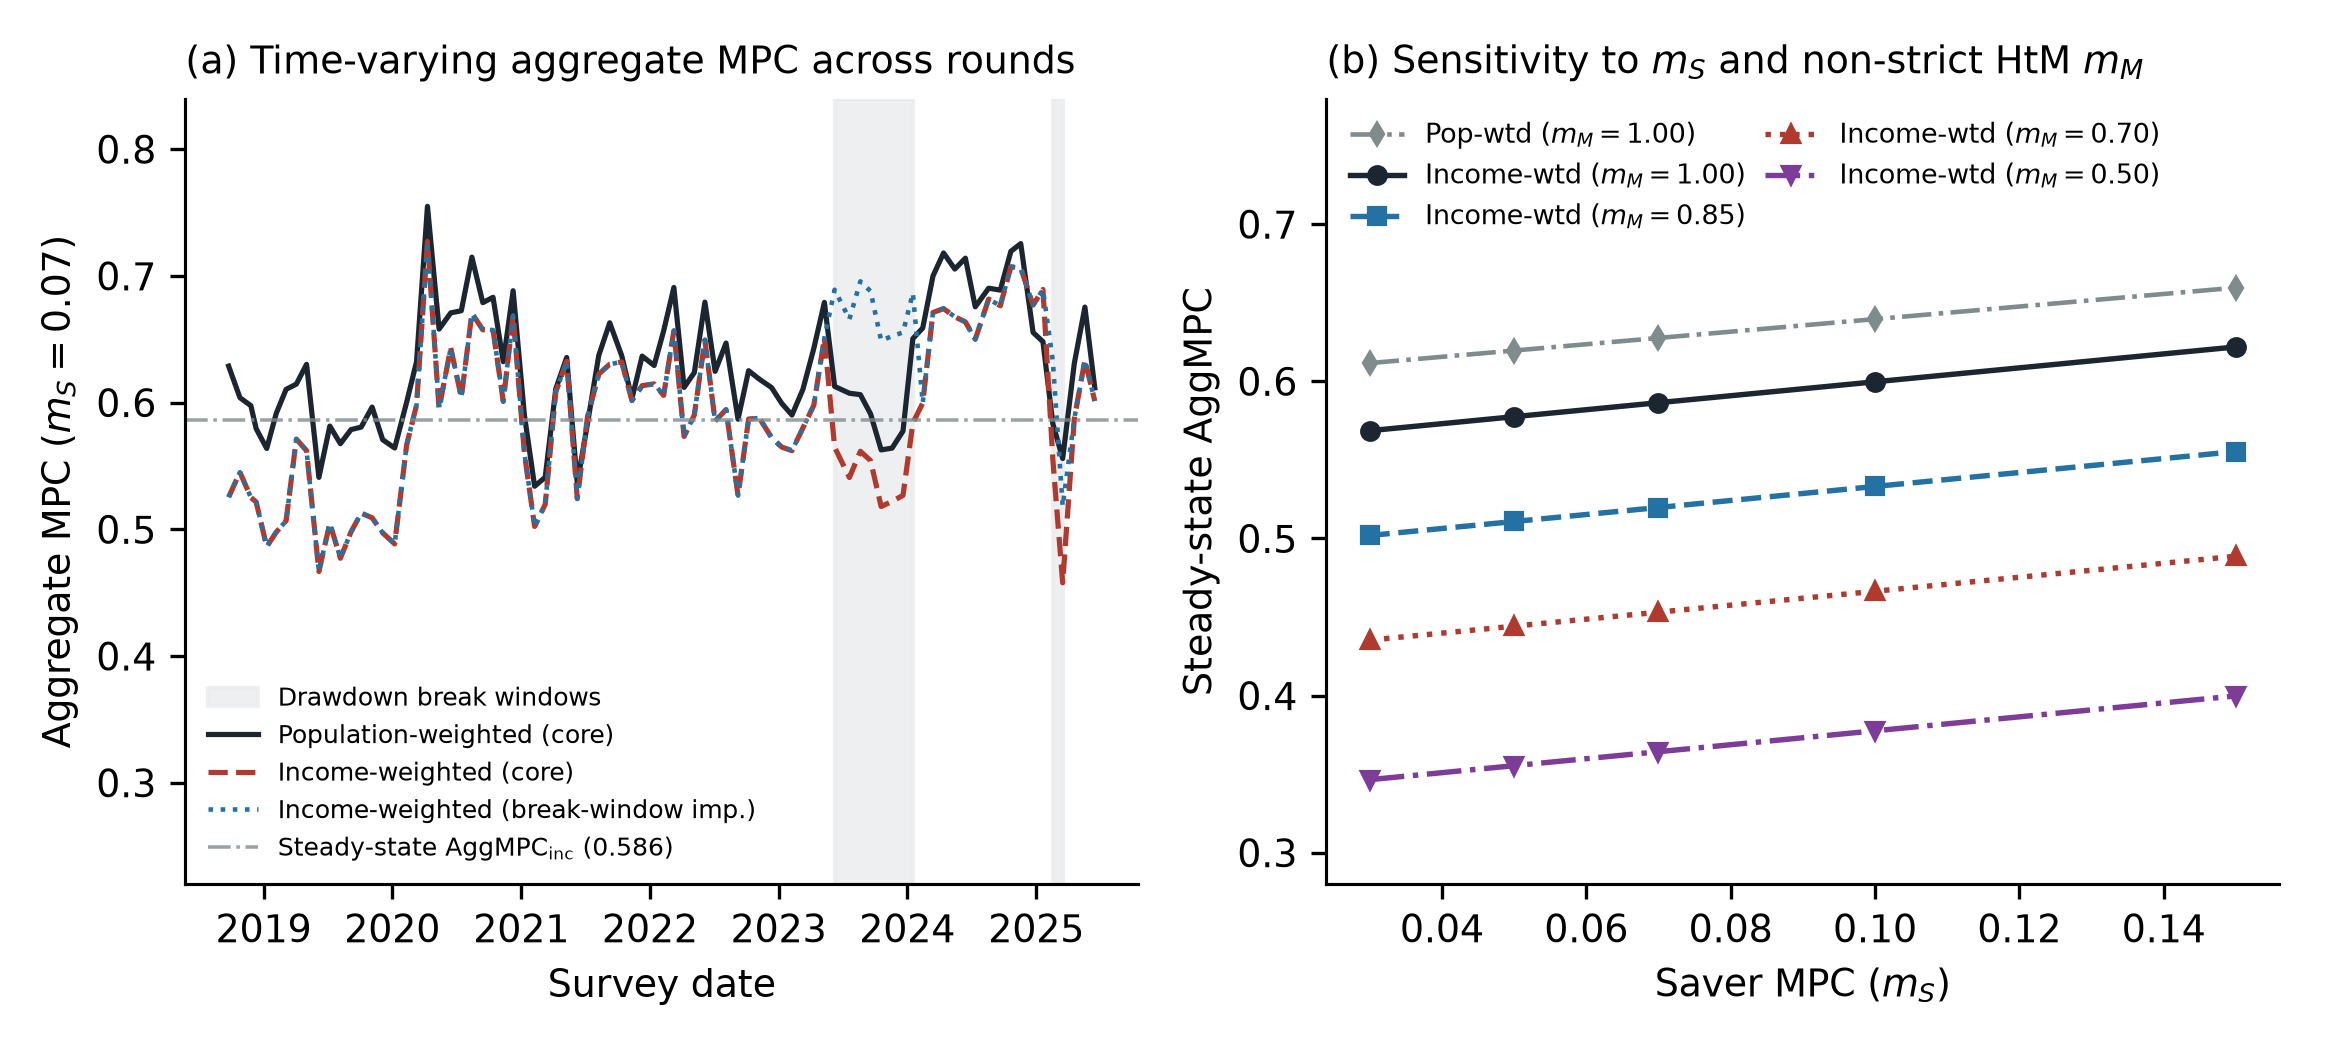
\includegraphics[width=0.96\linewidth]{../outputs/fig3_aggmpc_and_sensitivity.png}
\caption{Time-varying implied aggregate MPC and parameter sensitivity. Panel (a) plots population-weighted and income-weighted aggregate MPC across all 82 rounds under calibrated $(m_S, m_M, m_H) = (0.07, 1.00, 1.00)$ (core harmonized and break-window imputed; shaded bands mark drawdown-break windows). Panel (b) maps steady-state aggregate MPC across $m_S \in [0.03, 0.15]$ and $m_M \in \{0.50, 0.70, 0.85, 1.00\}$.}
\label{fig:aggmpc_sens}
\end{figure}

\begin{table}[tbp]
\centering
\caption{Sensitivity of steady-state aggregate MPC to saver ($m_S$) and non-strict HtM ($m_M$) parameters}
\label{tab:sens}
\small
\begin{tabular}{lccccc}
\toprule
 & $m_S = 0.03$ & $m_S = 0.05$ & $m_S = 0.07$ & $m_S = 0.10$ & $m_S = 0.15$ \\
\midrule
\multicolumn{6}{l}{\textit{Income-weighted $\text{AggMPC}_{\text{inc}}$ (proportional income shock)}} \\
$m_M = 1.00$ (baseline) & 0.569 & 0.578 & \textbf{0.586} & 0.600 & 0.622 \\
$m_M = 0.85$ & 0.502 & 0.511 & 0.520 & 0.533 & 0.555 \\
$m_M = 0.70$ & 0.435 & 0.444 & 0.453 & 0.466 & 0.489 \\
$m_M = 0.50$ & 0.347 & 0.355 & 0.364 & 0.378 & 0.400 \\
\midrule
\multicolumn{6}{l}{\textit{Population-weighted $\text{AggMPC}_{\text{pop}}$ (equal lump-sum transfer)}} \\
$m_M = 1.00$ (baseline) & 0.612 & 0.620 & \textbf{0.628} & 0.640 & 0.660 \\
$m_M = 0.85$ & 0.544 & 0.552 & 0.560 & 0.572 & 0.592 \\
$m_M = 0.70$ & 0.477 & 0.485 & 0.493 & 0.505 & 0.525 \\
$m_M = 0.50$ & 0.388 & 0.396 & 0.404 & 0.416 & 0.436 \\
\bottomrule
\end{tabular}
\begin{flushleft}
\footnotesize\textit{Notes:} Analytical steady-state pass-through from core harmonized $\pi = (0.400, 0.448, 0.152)$ and $\omega = (0.445, 0.444, 0.111)$ with $m_H = 1.00$. Under the post-r29 weighted HMM latent steady state $\pi^* = (0.343, 0.553, 0.104)$, baseline $(0.07, 1.00, 1.00)$ gives $\text{AggMPC}_{\text{inc}} = 0.647$ and $\text{AggMPC}_{\text{pop}} = 0.681$ (at $m_M = 0.85$: $\text{AggMPC}_{\text{inc}} = 0.566$ and $\text{AggMPC}_{\text{pop}} = 0.598$).
\end{flushleft}
\end{table}

\subsection{Dynamic IRFs, HMM persistence, job-loss targeting, and transfer rules}\label{sec:irf}

Figure~\ref{fig:irf_regimes} and Table~\ref{tab:counterfactuals} trace impulse responses to a uniform $-10.0\%$ persistent income shock ($\rho_z = 0.928$). Under the baseline smoothed-IBC rule, aggregate consumption drops $-5.83\%$ on impact and recovers monotonically to $-5.50\%$ at month 3 and $-4.06\%$ at month 12, reaching full 120-month present-value closure (1.000) with zero floor hits. Under raw noisy transitions $P$, two churn-driven artifacts appear: the pre-shock Saver cohort ($-0.70\%$ on impact) falls below the Strict-HtM cohort after month 4 ($-5.59\%$ versus $-4.68\%$ at month 6) because rapid monthly churn moves roughly half of initial savers into HtM within four months, and no-borrowing clawback produces a $-7.15\%$ month-3 hump with 148 floor hits. Replacing raw $P$ with the weighted post-round-29 HMM kernel $A^*$ eliminates the month-3 hump and cohort crossing: impact contraction widens to $-6.44\%$ (driven by the 0.657 latent broad-HtM share), the Saver cohort stays well above the Strict-HtM cohort at month 6 ($-4.01\%$ versus $-5.92\%$), and no-borrowing clawback declines monotonically ($-6.44\% \to -6.12\% \to -4.37\%$). Under clawback, rare floor hits increase from 148 to 256 in $A^*$ because longer saver spells allow larger accumulated negative asset deviations before an eventual switch into HtM triggers full clawback.

Saver expectations and macro regimes bound this baseline cleanly. In Panel (a), fixed-status PIH savers yield a $-5.67\%$ impact drop, while forward-looking buffer-stock iMPC savers respond more strongly and lift impact contraction to $-7.77\%$. Setting $r = 0$ (cash at home) or lowering $m_S$ to 0.03 barely shifts impact losses ($-5.83\%$ and $-5.65\%$), and break-window imputation gives $-5.96\%$. Across the five subperiod transition matrices in Panel (b), impact contractions widen from $-5.31\%$ before COVID-19 to $-6.12\%$ during COVID-19 and the late period.

\begin{figure}[tbp]
\centering
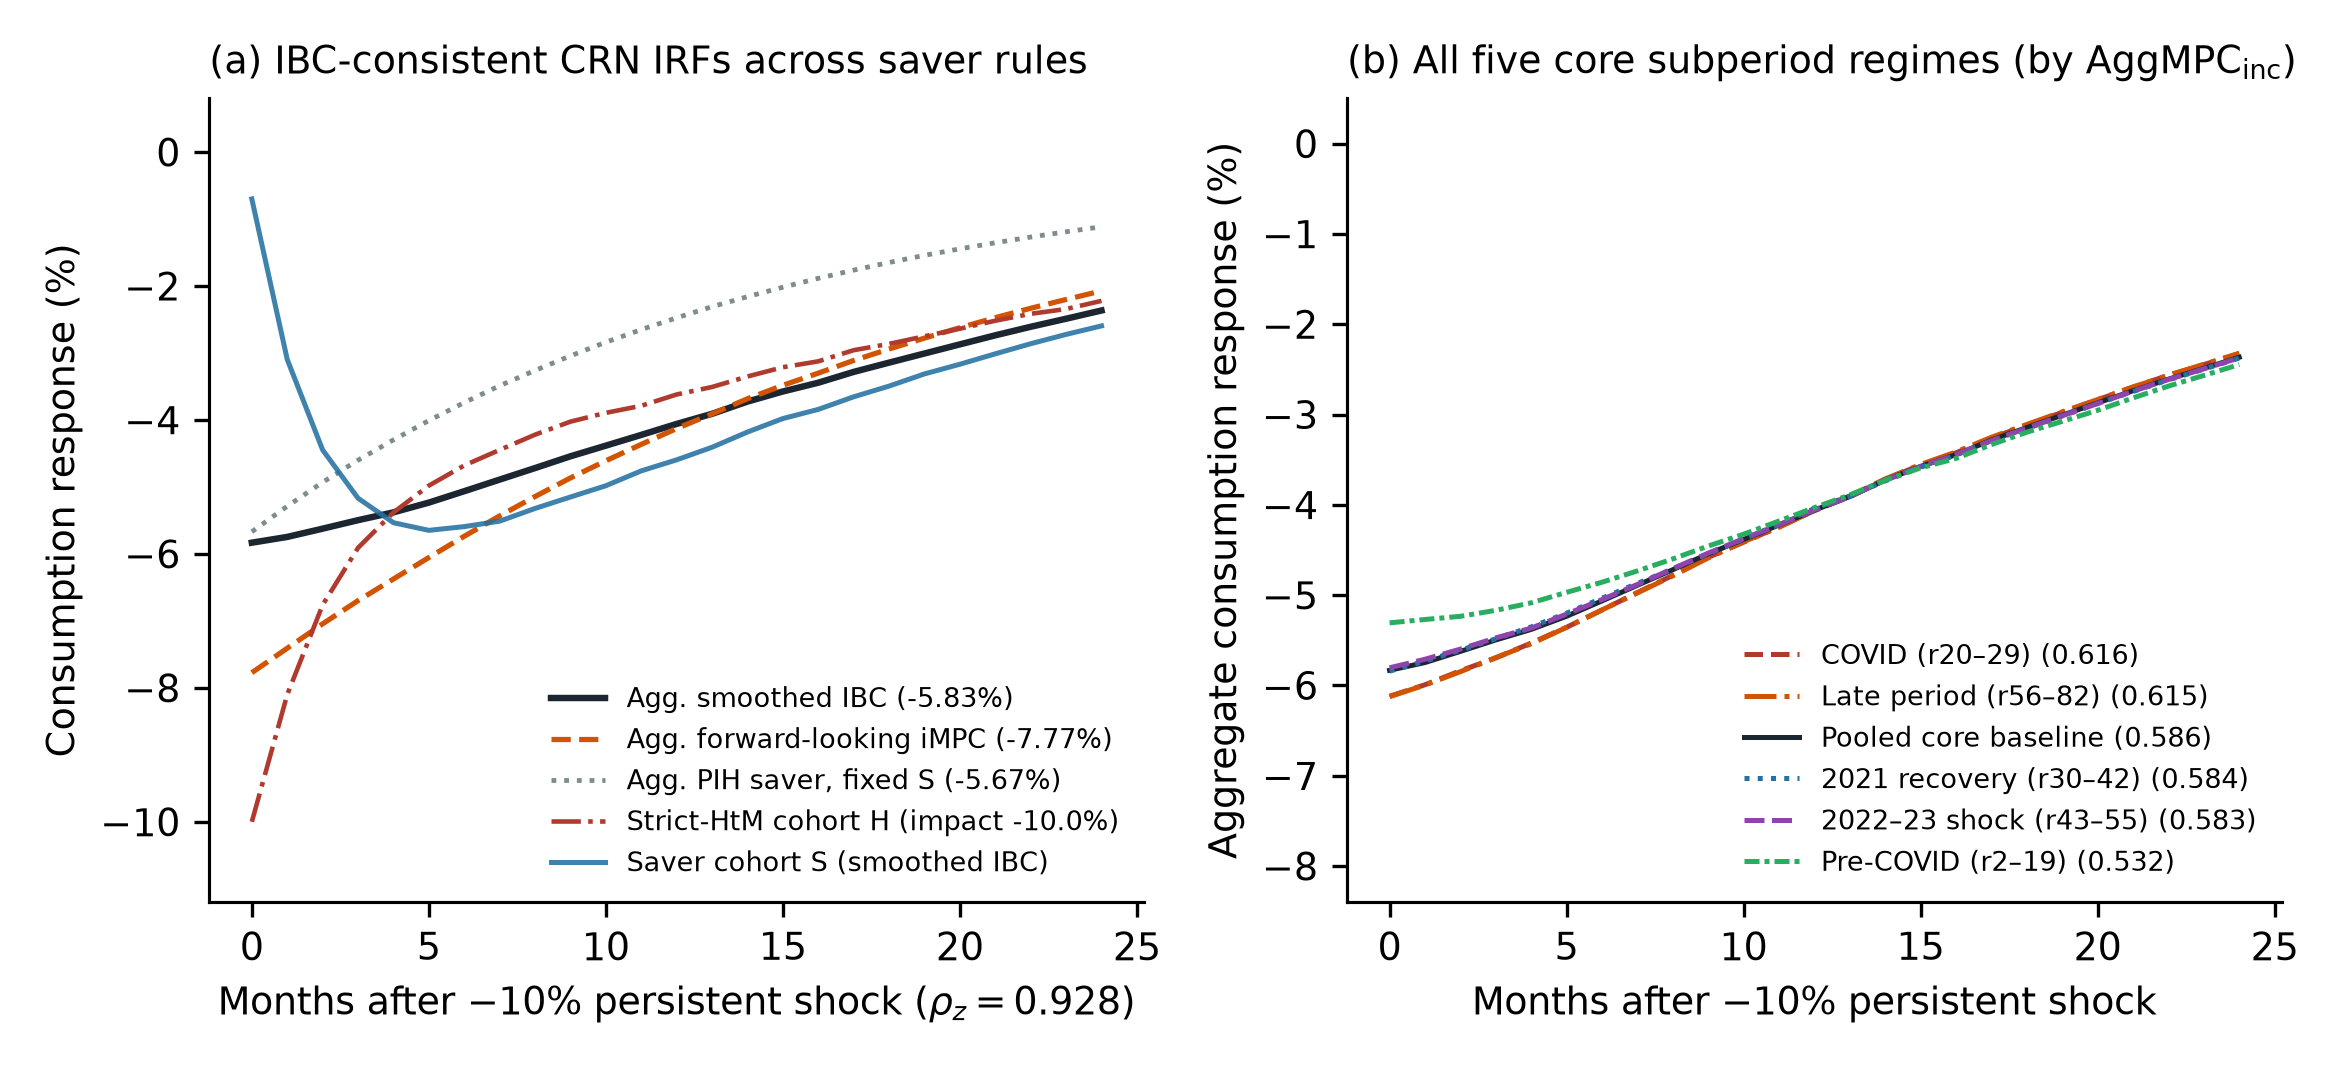
\includegraphics[width=0.96\linewidth]{../outputs/fig4_ibc_irfs_and_regimes.png}
\caption{IBC-consistent CRN impulse response functions to a uniform $-10\%$ persistent shock ($\rho_z = 0.928$). Panel (a) contrasts baseline smoothed-IBC aggregate consumption ($-5.83\%$ impact) against forward-looking iMPC ($-7.77\%$), fixed-status PIH ($-5.67\%$), and pre-shock Saver ($S$) and Strict-HtM ($H$) cohort paths. Panel (b) plots aggregate consumption IRFs across all five core subperiod transition matrices $P^{(r)}$.}
\label{fig:irf_regimes}
\end{figure}

\begin{figure}[tbp]
\centering
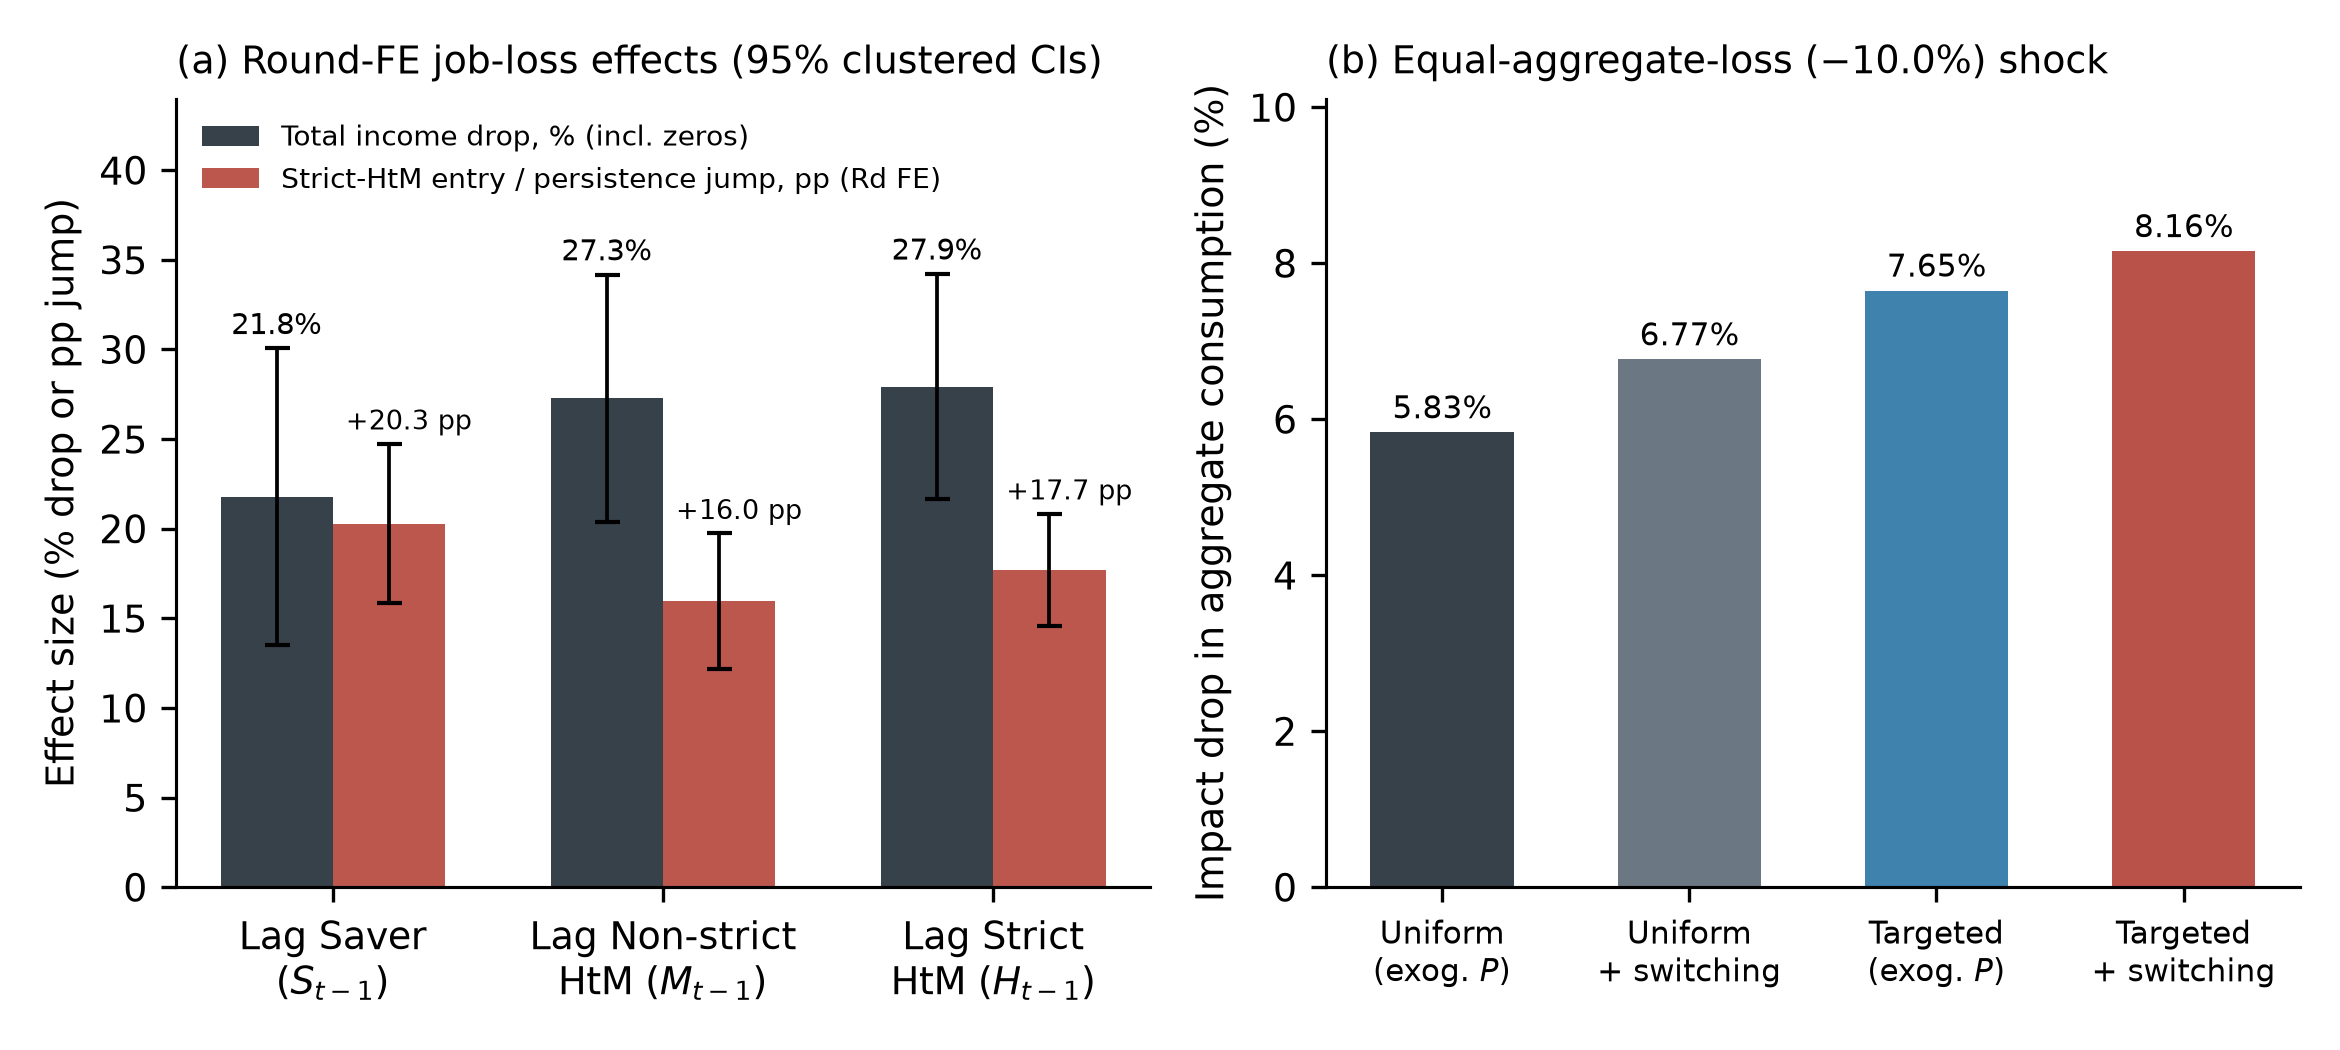
\includegraphics[width=0.96\linewidth]{../outputs/fig5_jobloss_and_amplification.png}
\caption{Job-loss gradients and equal-aggregate-loss shock amplification. Panel (a) summarizes Round-FE total real income drops (intensive plus extensive margins; 95\% CIs combine intensive and extensive clustered SEs) and strict-HtM entry/persistence jumps from Table~\ref{tab:workloss}. Panel (b) compares impact drops in aggregate consumption across four $-10.0\%$ aggregate shocks: uniform exogenous, uniform discrete with endogenous switching, targeted discrete by empirical job-loss exposure (exogenous $P$), and targeted discrete with endogenous switching.}
\label{fig:targeted}
\end{figure}

To quantify how much regressive job-loss exposure amplifies downturns \citep{patterson2023matching}, we run an equal-aggregate-loss discrete job-loss experiment holding total round-$t^*$ income contraction fixed at $-10.00\%$. Each state starts from its empirical job-loss rate $p^{\text{emp}} = (0.0107, 0.0152, 0.0524)$ and Round-FE total income loss $d = (21.8\%, 27.3\%, 27.9\%)$ from Table~\ref{tab:workloss}, with shocks entering $\delta_{i,t^*}$ and decaying at $\rho_z = 0.928$. Scaling recession intensity to $\kappa = 23.94$ gives discrete job-loss probabilities $p_s = \min(1, \kappa p_s^{\text{emp}}) = (25.6\%, 36.4\%, 100.0\%)$, which shrinks the saver share of total income losses from 44.5\% under a uniform hit to 25.1\% (25.3\% realized in finite-$N$ simulation; average state drops of $-5.64\%$ in $S$, $-9.90\%$ in $M$, and $-27.93\%$ in $H$). In the matched ``uniform discrete'' benchmark with switching, each state's job-loss probability is calibrated separately ($p_s^{\text{unif}} \approx 0.10 / d_s$) so every group loses $-10.00\%$ on impact.

Because 25.9\% of strict-HtM household-rounds rely solely on pensions, social benefits, or other non-labor income (weighted positive wage, self-employment, or agricultural earner shares are 80.8\% in $S$, 81.9\% in $M$, and 74.1\% in $H$), hitting a 100\% job-loss ceiling in $H$ is an upper bound. We therefore pair the baseline with two institutional bounds: (i) an \textit{earner-capped} $-10.00\%$ shock capping each state's job-loss probability at its empirical positive-earner share ($\kappa = 26.75$, giving $p = [28.6\%, 40.7\%, 74.1\%]$), and (ii) a milder \textit{uncapped} $-5.00\%$ shock ($\kappa = 11.01$, giving $p = [11.8\%, 16.7\%, 57.7\%]$, well below the 74.1\% earner ceiling). When endogenous switching is active, displaced savers enter $H$ ($+20.3$ pp) and $M$ ($+2.6$ pp) and displaced $M$ households enter $H$ ($+16.0$ pp); we also test the conservative HH+Round-FE switching slopes ($+14.6$ pp for $S$ and $+12.7$ pp for $M$) and re-run the targeted $-10.00\%$ shock under the persistent HMM kernel $A^*$ (a conservative check, since observed-state job-loss rates are attenuated by classification noise).

Figure~\ref{fig:targeted} and Table~\ref{tab:counterfactuals} split the resulting amplification into its channels:
\begin{itemize}
\item \textit{Pure matching amplification (exogenous transitions):} Shifting the $-10\%$ income hit from uniform to empirically targeted job losses deepens impact consumption losses from $-5.83\%$ to $-7.65\%$, a 1.31$\times$ multiplier (1.26$\times$ earner-capped, 1.33$\times$ on the uncapped $-5\%$ shock, 1.35$\times$ at $m_M = 0.85$, and 1.51$\times$ at $m_M = 0.50$).
\item \textit{Targeting with switching held fixed:} Because endogenous switching also amplifies a discrete uniform shock ($-6.77\%$ under Round-FE; $-6.44\%$ under HH-FE), holding switching constant isolates a targeting multiplier of 1.20$\times$ ($-8.16\%$ versus $-6.77\%$) under Round-FE, 1.24$\times$ ($-7.97\%$ versus $-6.44\%$) under HH-FE, 1.17$\times$ earner-capped, and 1.23$\times$ on the uncapped $-5\%$ shock.
\item \textit{Combined amplification and HMM persistence:} Combining regressive incidence with endogenous switching pushes impact contraction to $-8.16\%$, a 1.40$\times$ ratio over the exogenous-uniform baseline (1.37$\times$ under HH-FE, 1.36$\times$ earner-capped, 1.47$\times$ at $m_M = 0.85$, and 1.73$\times$ at $m_M = 0.50$). Under noisy $P$, rapid churn attenuates the gap over time (12-month cumulative $\Delta C / \Delta Y$ is 0.763 targeted versus 0.733 uniform). Under the persistent HMM kernel $A^*$, impact amplification starts at 1.23$\times$ exogenous ($-7.90\%$ versus $-6.44\%$) and 1.30$\times$ combined ($-8.36\%$), remains 1.20$\times$ at month 3 ($-7.03\%$ versus $-5.86\%$), and raises 12-month cumulative pass-through from 0.772 to 0.863 ($+11.9\%$).
\end{itemize}

Finally, we compare feasible fiscal transfer-targeting rules against universal lump-sum transfers drawn from the same stationary distribution ($\pi$ for raw $P$ and income proxies; $\pi^*$ for HMM kernels). At $(m_S, m_M, m_H) = (0.07, 1.00, 1.00)$, a universal transfer equal to $+1\%$ of aggregate income raises impact consumption by $+0.63\%$ ($\text{MPC} = 0.628$; $0.560$ at $m_M = 0.85$; $0.404$ at $m_M = 0.50$). Targeting the bottom income quintile (Q1) yields only a modest gain in pass-through, raising recipient MPC to 0.682 ($+8.6\%$; $+10.3\%$ at $m_M = 0.85$; $+16.4\%$ at $m_M = 0.50$), because 34.2\% of Q1 households report untouched savings. Targeting households observed in strict HtM three months earlier performs much better: under raw noisy $P$ (3-month strict-HtM retention 27.9\%), recipient MPC rises to 0.748 ($+19.2\%$; $+21.5\%$ at $m_M = 0.85$; $+29.7\%$ at $m_M = 0.50$). Under the weighted post-round-29 HMM, a policymaker observing $s_{t-3} = H$ through survey noise $E$ forms the Bayesian posterior $P(s^*_{t-3} \mid s_{t-3} = H) = (0.066, 0.255, 0.680)$, which propagates via $(A^*)^3$ to $(0.108, 0.316, 0.577)$ three months later. This feasible Bayesian rule delivers a recipient MPC of 0.900 against the matched HMM universal benchmark of 0.681 ($+32.2\%$; $+42.6\%$ at $m_M = 0.85$; $+83.6\%$ at $m_M = 0.50$), compared with an oracle latent-state ceiling of 0.951 ($+39.6\%$). The Q10-excluded HMM (+33.6\%) and break-window-imputed HMM (+27.2\%) yield similar lifts. As with latent spell lengths, these HMM targeting gains represent an upper bound if part of observed monthly churn reflects a genuinely volatile mover subgroup rather than pure reporting noise.

\begin{table}[tbp]
\centering
\caption{IBC-consistent CRN microsimulation counterfactuals ($N = 40{,}000$, $r = 0.0025$/mo)}
\label{tab:counterfactuals}
\scriptsize
\setlength{\tabcolsep}{2.2pt}
\resizebox{\linewidth}{!}{%
\begin{tabular}{lcccccccc}
\toprule
Experiment & Impact & Impact & $h = 3$ & $h = 12$ & 120m & Floor & \multicolumn{2}{c}{Impact $\Delta C$ ($h=0$)} \\
\cmidrule(lr){8-9}
 & $\Delta Y$ (\%) & $\Delta C$ (\%) & $\Delta C$ (\%) & $\Delta C$ (\%) & PV ratio & hits & $S$ cohort & $H$ cohort \\
\midrule
\multicolumn{9}{l}{\textit{Panel A: Uniform $-10\%$ persistent shocks across rules, kernels, and calibrations}} \\
\midrule
Smoothed IBC baseline ($m_S=0.07, m_M=1.00$) & $-10.00$ & $-5.83$ & $-5.50$ & $-4.06$ & 1.000 & 0 & $-0.70\%$ & $-10.00\%$ \\
No-borrowing clawback (raw $P$) & $-10.00$ & $-5.83$ & $-7.15$ & $-4.69$ & 1.000 & 148 & $-0.70\%$ & $-10.00\%$ \\
HMM latent kernel $A^*$ (post-r29, smoothed IBC) & $-10.00$ & $-6.44$ & $-5.86$ & $-4.09$ & 1.000 & 0 & $-0.70\%$ & $-10.00\%$ \\
HMM latent kernel $A^*$ (post-r29, clawback) & $-10.00$ & $-6.44$ & $-6.12$ & $-4.37$ & 1.000 & 256 & $-0.70\%$ & $-10.00\%$ \\
Forward-looking buffer-stock iMPC & $-10.00$ & $-7.77$ & $-6.70$ & $-4.13$ & 1.000 & 0 & $-5.03\%$ & $-10.00\%$ \\
Fixed-status PIH saver ($P = I$) & $-10.00$ & $-5.67$ & $-4.60$ & $-2.48$ & 0.669 & 0 & $-0.34\%$ & $-10.00\%$ \\
Low saver MPC ($m_S = 0.03$, qtrly 0.09) & $-10.00$ & $-5.65$ & $-4.95$ & $-3.30$ & 0.982 & 0 & $-0.30\%$ & $-10.00\%$ \\
Cash-at-home return ($r = 0$) & $-10.00$ & $-5.83$ & $-5.49$ & $-4.03$ & 1.000 & 0 & $-0.70\%$ & $-10.00\%$ \\
Lower non-strict MPC ($m_M = 0.85$) & $-10.00$ & $-5.17$ & $-5.08$ & $-4.03$ & 0.999 & 0 & $-0.70\%$ & $-10.00\%$ \\
Lower non-strict MPC ($m_M = 0.50$) & $-10.00$ & $-3.63$ & $-4.10$ & $-3.97$ & 0.999 & 0 & $-0.70\%$ & $-10.00\%$ \\
Break-window imputed $P$ & $-10.00$ & $-5.96$ & $-5.58$ & $-4.06$ & 1.000 & 0 & $-0.70\%$ & $-10.00\%$ \\
RANK benchmark ($m = 0.07$ all states) & $-10.00$ & $-0.70$ & $-2.26$ & $-3.87$ & 0.999 & 0 & $-0.70\%$ & $-0.70\%$ \\
\midrule
\multicolumn{9}{l}{\textit{Panel B: Equal-aggregate-loss discrete job-loss targeting and fiscal transfers}} \\
\midrule
Uniform discrete $-10\%$ + switching (Rd-FE) & $-10.00$ & $-6.77$ & $-5.72$ & $-4.13$ & 1.000 & 0 & $-2.79\%$ & $-10.00\%$ \\
Uniform discrete $-10\%$ + switching (HH-FE) & $-10.00$ & $-6.44$ & $-5.68$ & $-4.16$ & 1.000 & 0 & $-2.06\%$ & $-10.00\%$ \\
Targeted discrete $-10\%$ (exog.\ $P$, 1.31$\times$) & $-10.00$ & $-7.65$ & $-6.19$ & $-4.41$ & 1.000 & 0 & $-0.40\%$ & $-27.93\%$ \\
Targeted discrete $-10\%$ + Rd-FE switch (1.40$\times$) & $-10.00$ & $-8.16$ & $-6.25$ & $-4.36$ & 1.000 & 0 & $-1.52\%$ & $-27.93\%$ \\
Targeted discrete $-10\%$ + HH-FE switch (1.37$\times$) & $-10.00$ & $-7.97$ & $-6.23$ & $-4.38$ & 1.000 & 0 & $-1.11\%$ & $-27.93\%$ \\
Targeted discrete $-10\%$ earner-capped + Rd-FE (1.36$\times$) & $-10.00$ & $-7.95$ & $-6.05$ & $-4.26$ & 1.000 & 0 & $-1.72\%$ & $-20.64\%$ \\
Targeted discrete $-10\%$ HMM $A^*$ + Rd-FE (1.30$\times$) & $-10.00$ & $-8.36$ & $-7.03$ & $-4.25$ & 1.000 & 0 & $-1.62\%$ & $-27.93\%$ \\
Targeted discrete $-10\%$ ($m_M=0.85$, Rd-FE, 1.47$\times$) & $-10.00$ & $-7.59$ & $-5.75$ & $-4.32$ & 0.999 & 0 & $-1.50\%$ & $-27.93\%$ \\
Targeted discrete $-10\%$ ($m_M=0.50$, Rd-FE, 1.73$\times$) & $-10.00$ & $-6.26$ & $-4.59$ & $-4.23$ & 0.999 & 0 & $-1.45\%$ & $-27.93\%$ \\
Equal lump-sum transfer ($+1\%$ agg.\ $Y$) & $+1.00$ & $+0.63$ & $+0.02$ & $+0.01$ & 1.000 & 0 & $+0.06\%$ & $+1.37\%$ \\
\midrule
\multicolumn{9}{l}{\textit{Panel C: Core subperiod regimes (uniform $-10\%$ shock, smoothed IBC)}} \\
\midrule
Pre-COVID (r2--19, $\text{AggMPC}_{\text{inc}} = 0.532$) & $-10.00$ & $-5.31$ & $-5.17$ & $-4.03$ & 1.000 & 0 & $-0.70\%$ & $-10.00\%$ \\
2022--23 shock (r43--55, $\text{AggMPC}_{\text{inc}} = 0.583$) & $-10.00$ & $-5.80$ & $-5.47$ & $-4.06$ & 1.000 & 0 & $-0.70\%$ & $-10.00\%$ \\
2021 recovery (r30--42, $\text{AggMPC}_{\text{inc}} = 0.584$) & $-10.00$ & $-5.84$ & $-5.48$ & $-4.04$ & 1.000 & 0 & $-0.70\%$ & $-10.00\%$ \\
COVID (r20--29, $\text{AggMPC}_{\text{inc}} = 0.616$) & $-10.00$ & $-6.12$ & $-5.70$ & $-4.06$ & 1.000 & 0 & $-0.70\%$ & $-10.00\%$ \\
Late period (r56--82, $\text{AggMPC}_{\text{inc}} = 0.615$) & $-10.00$ & $-6.12$ & $-5.69$ & $-4.06$ & 1.000 & 0 & $-0.70\%$ & $-10.00\%$ \\
\bottomrule
\end{tabular}%
}
\begin{flushleft}
\footnotesize\textit{Notes:} All simulations use $N = 40{,}000$, seed 12345, CRN across baseline and shocked paths, and $(m_S, m_M, m_H) = (0.07, 1.00, 1.00)$ unless noted. RANK denotes the representative-agent New Keynesian benchmark. ``Floor hits'' counts post-shock household-months (excluding burn-in) where $y^{\text{base}} + \Delta c < 0$. In Panel A, fixed-status PIH savers amortize over an infinite horizon and consume $1 - (1+r)^{-121} = 26.1\%$ of their shock PV across $h = 0, \dots, 120$, yielding an aggregate 120m PV ratio of $1 - 0.448 \times (1 - 0.261) = 0.669$ given realized saver income share $0.448$ (asymptotically 1.000). In Panel B, holding switching fixed isolates a targeting multiplier of 1.20$\times$ (Rd-FE), 1.24$\times$ (HH-FE), 1.17$\times$ (earner-capped, $p_H \le 74.1\%$), and 1.16$\times$ (HMM $A^*$, where exogenous targeting gives $-7.90\%$ or 1.23$\times$); an uncapped $-5.0\%$ shock ($\kappa = 11.01$, $p_H = 57.7\%$) yields 1.33$\times$ exogenous, 1.23$\times$ holding switching fixed, and 1.42$\times$ combined amplification.
\end{flushleft}
\end{table}

\FloatBarrier
\section{Policy Implications, Limitations, and Concluding Remarks}\label{sec:limits}

\subsection{Policy implications for macroeconomic stabilization in Uzbekistan}\label{sec:policy}

Three policy lessons follow for macroeconomic and social policy in Uzbekistan and comparable cash-intensive transition economies:

\begin{enumerate}
\item \textit{Distress-based transfer targeting outperforms income cutoffs.} Strict-HtM families earn 34.2\% less than savers, face four to five times higher job-loss risk even at two- to three-month lags, and remain vulnerable over multi-quarter horizons once survey noise is filtered out (83.9\% latent three-month retention). Consistent with developing-country evidence on high transfer pass-through \citep{egger2022general}, simple bottom-quintile income targeting raises impact recipient MPC by only 8.6\% above a universal transfer (0.682 versus 0.628; +16.4\% at $m_M = 0.50$). Targeting households flagged with financial distress three months earlier raises pass-through by 19.2\% under raw transitions (0.748 versus 0.628; +29.7\% at $m_M = 0.50$) and by 32.2\% under feasible Bayesian updating in the post-round-29 HMM (0.900 versus 0.681; +42.6\% at $m_M = 0.85$ and +83.6\% at $m_M = 0.50$, subject to the mover--stayer caveat above). Extending temporary eligibility in Uzbekistan's Unified Social Protection Registry to recently displaced workers also cushions the 14.6--22.9 percentage-point jump in broad-HtM entry among job-losing savers.
\item \textit{Direct household interest-rate substitution has limited reach.} With roughly 60\% of households reporting no savings or active hard coping (60.6\%--70.3\% across weighted HMM specifications) and 94.8\% of realized savers holding zero-interest cash at home, standard Euler-equation substitution acts on a minority of aggregate spending. Although we do not estimate monetary transmission directly, these balance-sheet facts imply that CBU policy rates are likely to transmit mainly through indirect credit, exchange-rate, and labor-income channels rather than direct household deposit substitution.
\item \textit{Existing payment cards can anchor formal liquid saving.} By June 2025, 85.1\% of weighted Uzbek households held a bank card and at least 95\% of cardholders used them routinely for transfers, purchases, and ATM withdrawals, yet only 3.1\% of realized savers kept money in bank deposits. Attaching simple, positive-real-yield liquid savings pockets directly to existing payroll and pension cards, paired with transparent deposit-insurance communication, aids both financial inclusion and macroeconomic stabilization by expanding household liquid buffers.
\end{enumerate}

\subsection{Limitations and concluding remarks}\label{sec:concl}

Five caveats bound what can be inferred from these data. First, L2CU contains neither a total-consumption diary nor liquid-asset balances. State-level MPCs are therefore calibrated across an explicit grid ($m_S \in [0.03, 0.15]$, $m_M \in [0.50, 1.00]$) rather than estimated directly, and the 94.8\% cash-at-home saving share rules out a formal balance-sheet test of wealthy hand-to-mouth households \citep{kaplan2014wealthy}. Second, public L2CU releases omit PSU, stratum, and regional identifiers, confining the analysis to national totals and leaving Kish within-round standard errors unadjusted for geographic clustering. Third, while official metadata and our forensic checks isolate discontinuities at rounds 29, 44, 58--65, 76, and 78--79, round-specific CATI routing scripts are unavailable publicly, and falling realized-saving reports point to late-panel respondent fatigue. Fourth, our microsimulation holds prices and wages fixed with exogenous Markov transitions; embedding these moments in a general-equilibrium HANK model with endogenous precautionary saving, import leakage, and nominal rigidities remains an open next step. Fifth, small monthly counts of job-losing remittance recipients limit statistical power for cross-border insurance tests, even though adding remittance inflows leaves aggregate income shares unchanged.

Across 82 consecutive monthly waves, roughly 60\% of Uzbek households (61.3\% under break-window imputation and 60.6\%--70.3\% across weighted HMM specifications) report no liquid savings or rely on hard coping in a typical month. Underlying liquidity states persist for 15 to 44 months, and non-strict HtM households show clearly elevated financial vulnerability relative to savers. Under calibrated state MPCs, steady-state aggregate pass-through sits at 0.59--0.63 at $m_M = 1.00$ (0.52--0.56 at $m_M = 0.85$; 0.36--0.40 at $m_M = 0.50$), peaking sharply in April 2020. Because job loss strikes strict-HtM households four to five times as often as savers even at two- to three-month lags and pushes displaced savers into HtM status, uniform-shock exercises understate impact consumption contractions by 26\%--31\% under exogenous transitions, 17\%--24\% holding switching fixed, and 30\%--40\% jointly across raw, earner-capped, and HMM kernels (rising to 73\% at $m_M = 0.50$). Adding a compact quarterly expenditure module, cash-buffer brackets, and hypothetical windfall-MPC questions \citep{jappelli2014fiscal,fuster2021what} to future L2CU waves would allow researchers to estimate state-specific MPCs directly.

\section*{Declarations}

\noindent\textbf{Funding:} No external funding was received for conducting this study.

\medskip\noindent\textbf{Competing interests:} The author declares no financial or non-financial competing interests relevant to this article.

\medskip\noindent\textbf{Data availability:} Household microdata are publicly available to registered researchers via the World Bank Microdata Library (Listening to Citizens of Uzbekistan Survey 2018--2025, v03, Catalog 6412, \url{https://microdata.worldbank.org/index.php/catalog/6412}). Official monthly consumer price indices are openly available from the Statistics Agency under the President of the Republic of Uzbekistan (\url{https://siat.stat.uz}, Tables 1285 and 1286).

\medskip\noindent\textbf{Code availability:} All Python scripts required to reproduce every table, simulation, and figure from the source data are publicly available at \url{https://github.com/azimovu/uzbekistan-hank-lite} (Release v1.0.0) and archived on Zenodo.

\medskip\noindent\textbf{Ethical approval and informed consent:} This study performs secondary statistical analysis of fully anonymized, publicly released World Bank microdata; no new human-subjects data were collected.

\clearpage
\appendix
\section{L2CU Variable Mapping}\label{app:dict}

Table~\ref{tab:dict} maps manuscript concepts to exact variable names in the World Bank L2CU v03 public archive and Catalog 6412 metadata \citep{WB2025L2CU}.

\begin{table}[htbp]
\centering
\caption{Data dictionary mapping manuscript variables to L2CU v03 fields}
\label{tab:dict}
\scriptsize
\setlength{\tabcolsep}{2.2pt}
\begin{tabular}{lll}
\toprule
Manuscript concept & L2CU file & Exact field name(s) \\
\midrule
Sampling weight & Household & \texttt{popw} \\
Household size & Household & \texttt{hhsize} \\
Cash income (6 components) & Household & \texttt{wage\_amount}, \texttt{aginc\_amount}, \texttt{selfempinc\_amount}, \\
 & & \texttt{otherinc\_amount}, \texttt{pension\_amount}, \texttt{benefit\_amount} \\
Savings buffer / drawdown (Q8, 30d) & Household & \texttt{savings\_past30d} (``Do not have any savings'', ``No'', ``Yes'') \\
Hard coping: loan, assets, food cut (30d) & Household & \texttt{loan\_past30d} (Q7), \texttt{assets\_past30d} (Q9), \texttt{consumption\_past30d} (Q10) \\
Food-money sufficiency (Q5, 30d) & Household & \texttt{food\_past30d} (``No'' = insufficient) \\
Utility arrears, medical delay, econ.\ cond. & Household & \texttt{utility\_past30d} (Q6), \texttt{medical\_past30d} (Q11), \texttt{economic\_condition} \\
Financial change (Q1, 30d) & Household & \texttt{finance\_30d\_ago} (case-insensitive ``worse'') \\
FIES food insecurity (r49--82) & Household & \texttt{ln\_1} through \texttt{ln\_8} (any ``Yes'') \\
Realized past-30d saving \& storage form$^\dagger$ & Household & \texttt{saving\_next30d}, \texttt{deposit\_amount}, \texttt{deposit\_form} \\
Bank-card ownership \& usage (30d) & Household & \texttt{bank\_card\_hh}, \texttt{bank\_receive\_past30d}, \\
 & & \texttt{bank\_purchase\_past30d}, \texttt{bank\_atm\_past30d} \\
7-day staple items & Household & \texttt{bread\_past7d\_cost}, \texttt{flour\_past7d\_cost} \\
Household job-loss indicator & Individual & \texttt{work\_lost\_hh} (aggregated to any ``Yes'' per household-round) \\
Individual demographics \& work & Individual & \texttt{age}, \texttt{gender}, \texttt{education}, \texttt{work\_type\_new} \\
Migrant \& non-member remittances & Individual & \texttt{mig\_living\_remittance}, \texttt{mig\_living\_remittance\_amount}, \\
 & & \texttt{mig\_living\_remittance\_currency}, \texttt{mig\_living\_remittance\_use}, \\
 & & \texttt{remittance\_hh\_amount}, \texttt{remittance\_hh\_currency} \\
\bottomrule
\end{tabular}
\begin{flushleft}
\footnotesize\textit{Notes:} $^\dagger$Despite its column name in the public v03 file, \texttt{saving\_next30d} acts as the exact skip-pattern filter for realized past-30-day saving details (\texttt{deposit\_amount} and \texttt{deposit\_form} are populated for all 3,429 \texttt{saving\_next30d == "Yes"} observations and zero \texttt{"No"} observations).
\end{flushleft}
\end{table}

\section{Replication Summary}\label{app:rep}
\begingroup\sloppy\small
All empirical moments, tables, simulations, and figures reproduce from a self-contained Python replication archive (standard library for scripts 01--05 and 07; \texttt{matplotlib} for script 06) using the public World Bank L2CU v03 archive (\texttt{UZB\_2018-2025\_L2CU\_v03\_M\_CSV.zip}) and Statistics Agency of Uzbekistan CPI files (\texttt{sdmx\_cpi\_1285.csv}, \texttt{sdmx\_cpi\_1286.csv}). Running \texttt{./replication/run\_all.sh} executes the national HtM series and forensic audit (\texttt{01}), transitions and regimes (\texttt{02}), income gaps and lag-12/24/48/agricultural PPT (\texttt{03}), Round/HH-FE job-loss regressions (\texttt{04}), weighted HMM misclassification (core, post-trough, break-window-imputed, and Q10-excluded), $M_1$ validation, lagged $t-2/t-3$ exposure, event study, refresh/spillover/job-loss audits, earner shares, and remittance checks (\texttt{07}), CRN IBC microsimulation across $m_M \in [0.50, 1.00]$ including earner-capped and HMM-kernel targeting (\texttt{05}), and 300-DPI figures (\texttt{06}).
\endgroup

\clearpage
\bibliographystyle{plainnat}
\bibliography{refs_ecop}

\end{document}
